\documentclass[]{usiinfbachelorproject}

\usepackage{todonotes}
\usepackage{soul}
\usepackage{dirtytalk}
\usepackage[nottoc]{tocbibind}

\captionsetup{labelfont={bf}}
%\setlength{\parindent}{0cm}

\author{Davide Ciulla}

\title{Stack and Heap Diagrams}
\subtitle{A Graphical Editor}
\versiondate{\today}

\begin{committee}
%With more than 1 advisor an error is raised...: only 1 advisor is allowed!
\advisor[Universit\`a della Svizzera Italiana, Switzerland]{Prof.}{Matthias}{Hauswirth}
%You can comment out  these lines if you don't have any assistant
%\assistant[Universit\`a della Svizzera Italiana, Switzerland]{Title}{AssistantName1}{AssistanSurname1}
%\assistant[Universit\`a della Svizzera Italiana, Switzerland]{Title}{AssistantName2}{AssistanSurname2}
\end{committee}

\abstract{
Teaching students the fundamentals of programming is not an easy task at all, but luckily there are useful tools like Stack and Heap diagrams that can facilitate this process, by providing professors ways to easily assess the students understanding on a given topic. However, these diagrams are often drawn either on paper or with legacy software that must be installed on the computer. In this project, I developed a web-based stack and heap graphical editor, using modern front-end web technologies like React and Sass.}



\begin{document}

\maketitle


\tableofcontents
\newpage


%%%%%%%%%%%%%%%%%%%%%%%%%
\section{Introduction} \label{introduction}
%%%%%%%%%%%%%%%%%%%%%%%%%

In this first section I am going to describe all the thoughts that went into this project at the very early stages, from the moment I first discussed the project with prof. Hauswirth, to the moment right before starting the pre-production phase (see \hyperref[requirements+analysis]{\textbf{Section 3}}).

\subsection{Theoretical Background}

Before continuing, I need to clarify some theoretical concepts that will be used many times throughout this report. In particular stack and heap, notional machines and clicker tools.

\subsubsection{Stack and heap}
In the world of computer science, stack and heap are two very important memory allocation areas. The stack is a LIFO (\emph{Last In First Out}) data structure responsible for keeping track of function calls. Every time a function is called, a new stack frame is pushed onto the stack, containing its parameters, its local variables
 and the return address \footnote{\url{https://medium.com/fhinkel/confused-about-stack-and-heap-2cf3e6adb771}}. Stack frames only exist during the execution of a function, and are popped from the stack when the latter has completed its lifecycle.\\
 Conversely, the heap does not have a LIFO structure and it is independent from the program execution, being a segment of memory dedicated to dynamic memory allocation. When we program and allocate memory, we create objects on the heap. These objects do not disappear automatically like stack frames, and in some programming languages (like C and C++) they must be manually deallocated by the programmer (bad heap management can cause memory leaks - a failure in a program to release discarded memory, causing impaired performance or failure. \footnote {\url{https://en.wikipedia.org/wiki/Memory_leak}}).\\
 
\begin{figure}[h!]
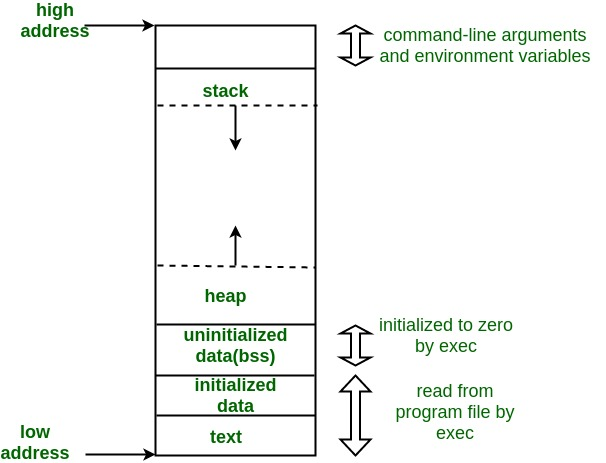
\includegraphics[scale=0.4]{figures/memory_layout.jpg}
\centering
\caption {Generalized memory layout of a program}
\end{figure}
 
\subsubsection{Notional machines}

A notional machine can be described as a set of abstractions that define the structure and behavior of a computational device \cite{guzdial_et_al:DR:2019:11627}. The goal of such a machine is not to be an exact replica of the real device, because by providing abstractions it is hopefully easier for students to understand the real machine \cite{7743153}.\\
\noindent Students build their mental models about the notional machine through teaching, learning methods and materials used in programming classes \cite{HIDALGO-CESPEDES2016}.
 
\begin{figure}[h!]
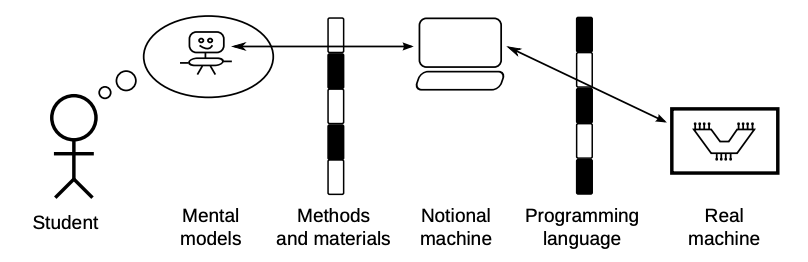
\includegraphics[scale=0.8]{figures/notional_machine.png}
\centering
\caption {Process of creating mental models about notional machines.}
\end{figure}
 
\vspace{\fill}
\pagebreak
 
\subsubsection{Clicker tools}
 
According to the Luce Group\footnote{\url{http://luce.inf.usi.ch/}}, "a clicker is a special purpose remote control used in traditional group response systems, where an instructor projects a multiple-choice question on the classroom projector and students use these tools to submit their answers by pressing one of the buttons. The advantage of using such systems is that the instructor has immediate feedback on the students understanding, by seeing their responses aggregated in the form of a histogram." \footnote{\url{http://sape.inf.usi.ch/informa}}
 
\subsection{Motivation}

As I am going to show in \hyperref[state]{\textbf{Section 2}} about state-of-the-art projects for programs visualizations, one can do a quick Google search and see that there are already tools in the real world that help students grasp important computer science topics, by showing the state of their code at each point of its execution.\\
However, the majority of them are automated, meaning that they take real code as input and automatically create diagrams as outputs. With such programs, \textbf{students cannot demonstrate their understanding}, and \emph{that} is exactly why I am making this application.

\subsection{Goal} \label{goal}

The goal of this project is to create a web application inspired by the Informa clicker tool, that allows students to very easily create Stack and Heap diagrams to visualize the structure of their code and better understand what is actually happening under the hood. This kind of diagram can give very useful insights both to the student and to the professor.\\ This application is planned to be integrated into Informa (prof. Hauswirth's web platform for his Programming Fundamentals 2 course), but it can also be used as a standalone application. That way, students can not only use it in class during class exercises, but also for instance at home while studying on their own.\\
Furthermore, a JavaScript object containing the data representation of the diagram is constantly kept up-to-date with every state change happening, which can be used for automatic testing and potentially instant feedback on the correctness of their diagrams.

\subsection{Use cases}

This application was developed with the two following use cases in mind:

\begin{enumerate}
\item Teacher provides some code and an arbitrary breakpoint, and the student must create  a diagram mirroring the state of the program when the breakpoint is reached.
\item Teacher draws a diagram and student must be able to describe the current state of the program execution.
\end{enumerate}

\vspace{\fill}
\pagebreak

%%%%%%%%%%%%%%%%%%%%%%%%%
\section{State of the Art} \label{state}
%%%%%%%%%%%%%%%%%%%%%%%%%

In this section I am going to showcase projects that I consider to be state-of-the-art in terms of visual representations of code. Not all of them are related to stack and heap diagrams, but they do still set a benchmark for graphical output and ease of learning.

\subsection{Informa Clicker - Luce Group}

\noindent Informa \footnote{\url{https://informa.inf.usi.ch/}} is not only a teaching platform, but it also has a clicker tool available for download, that students can use to solve interactive problems. One of the problems they can solve is showing the correct state of a Stack and Heap Diagram at a given point of a code execution.\\

\noindent This clicker tool was developed by professor Matthias Hauswirth, my bachelor thesis advisor, for the Luce Group.

\begin{figure}[h!]
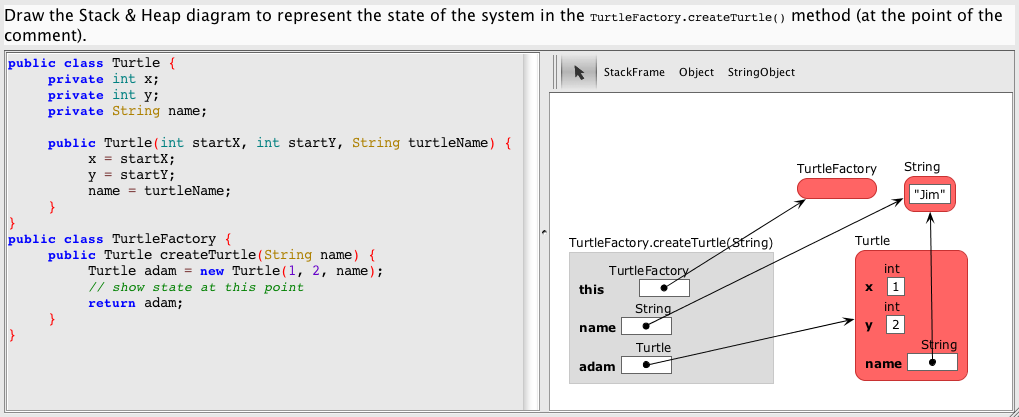
\includegraphics[scale=0.4]{figures/informa_clicker.png}
\centering
\caption {Stack and Heap Diagrams in the Informa clicker tool}
\end{figure}

\subsection{BlueJ - King's College London}

BlueJ \footnote{\url{https://www.bluej.org/}} (see \hyperref[bluej_classes_objects]{\textbf{Figure 4}} and \hyperref[bluej_objects_open]{\textbf{Figure 5}}) is free Java IDE (\emph{Integrated Development Environment}) designed for beginners, developed by the King's College London and officially supported by Oracle, the company that owns the Java platform.
The aspect that makes BlueJ stand out from the other IDEs is its powerful main view, which shows an interactive diagram of the different elements that compose your source code. It also renders arrows that are very useful, because they show how the different classes are interconnected. Objects are shows too, but they do not present any arrow.\\
BlueJ is also used in the textbook \emph{Objects First with Java: A Practical Introduction using BlueJ} by David J. Barnes \& Michael K\"{o}lling \cite{barnes2016objects}, a popular choice for programming fundamentals classes that use Java as the first step into the world of object oriented programming languages.

\begin{figure}[h]
\centering
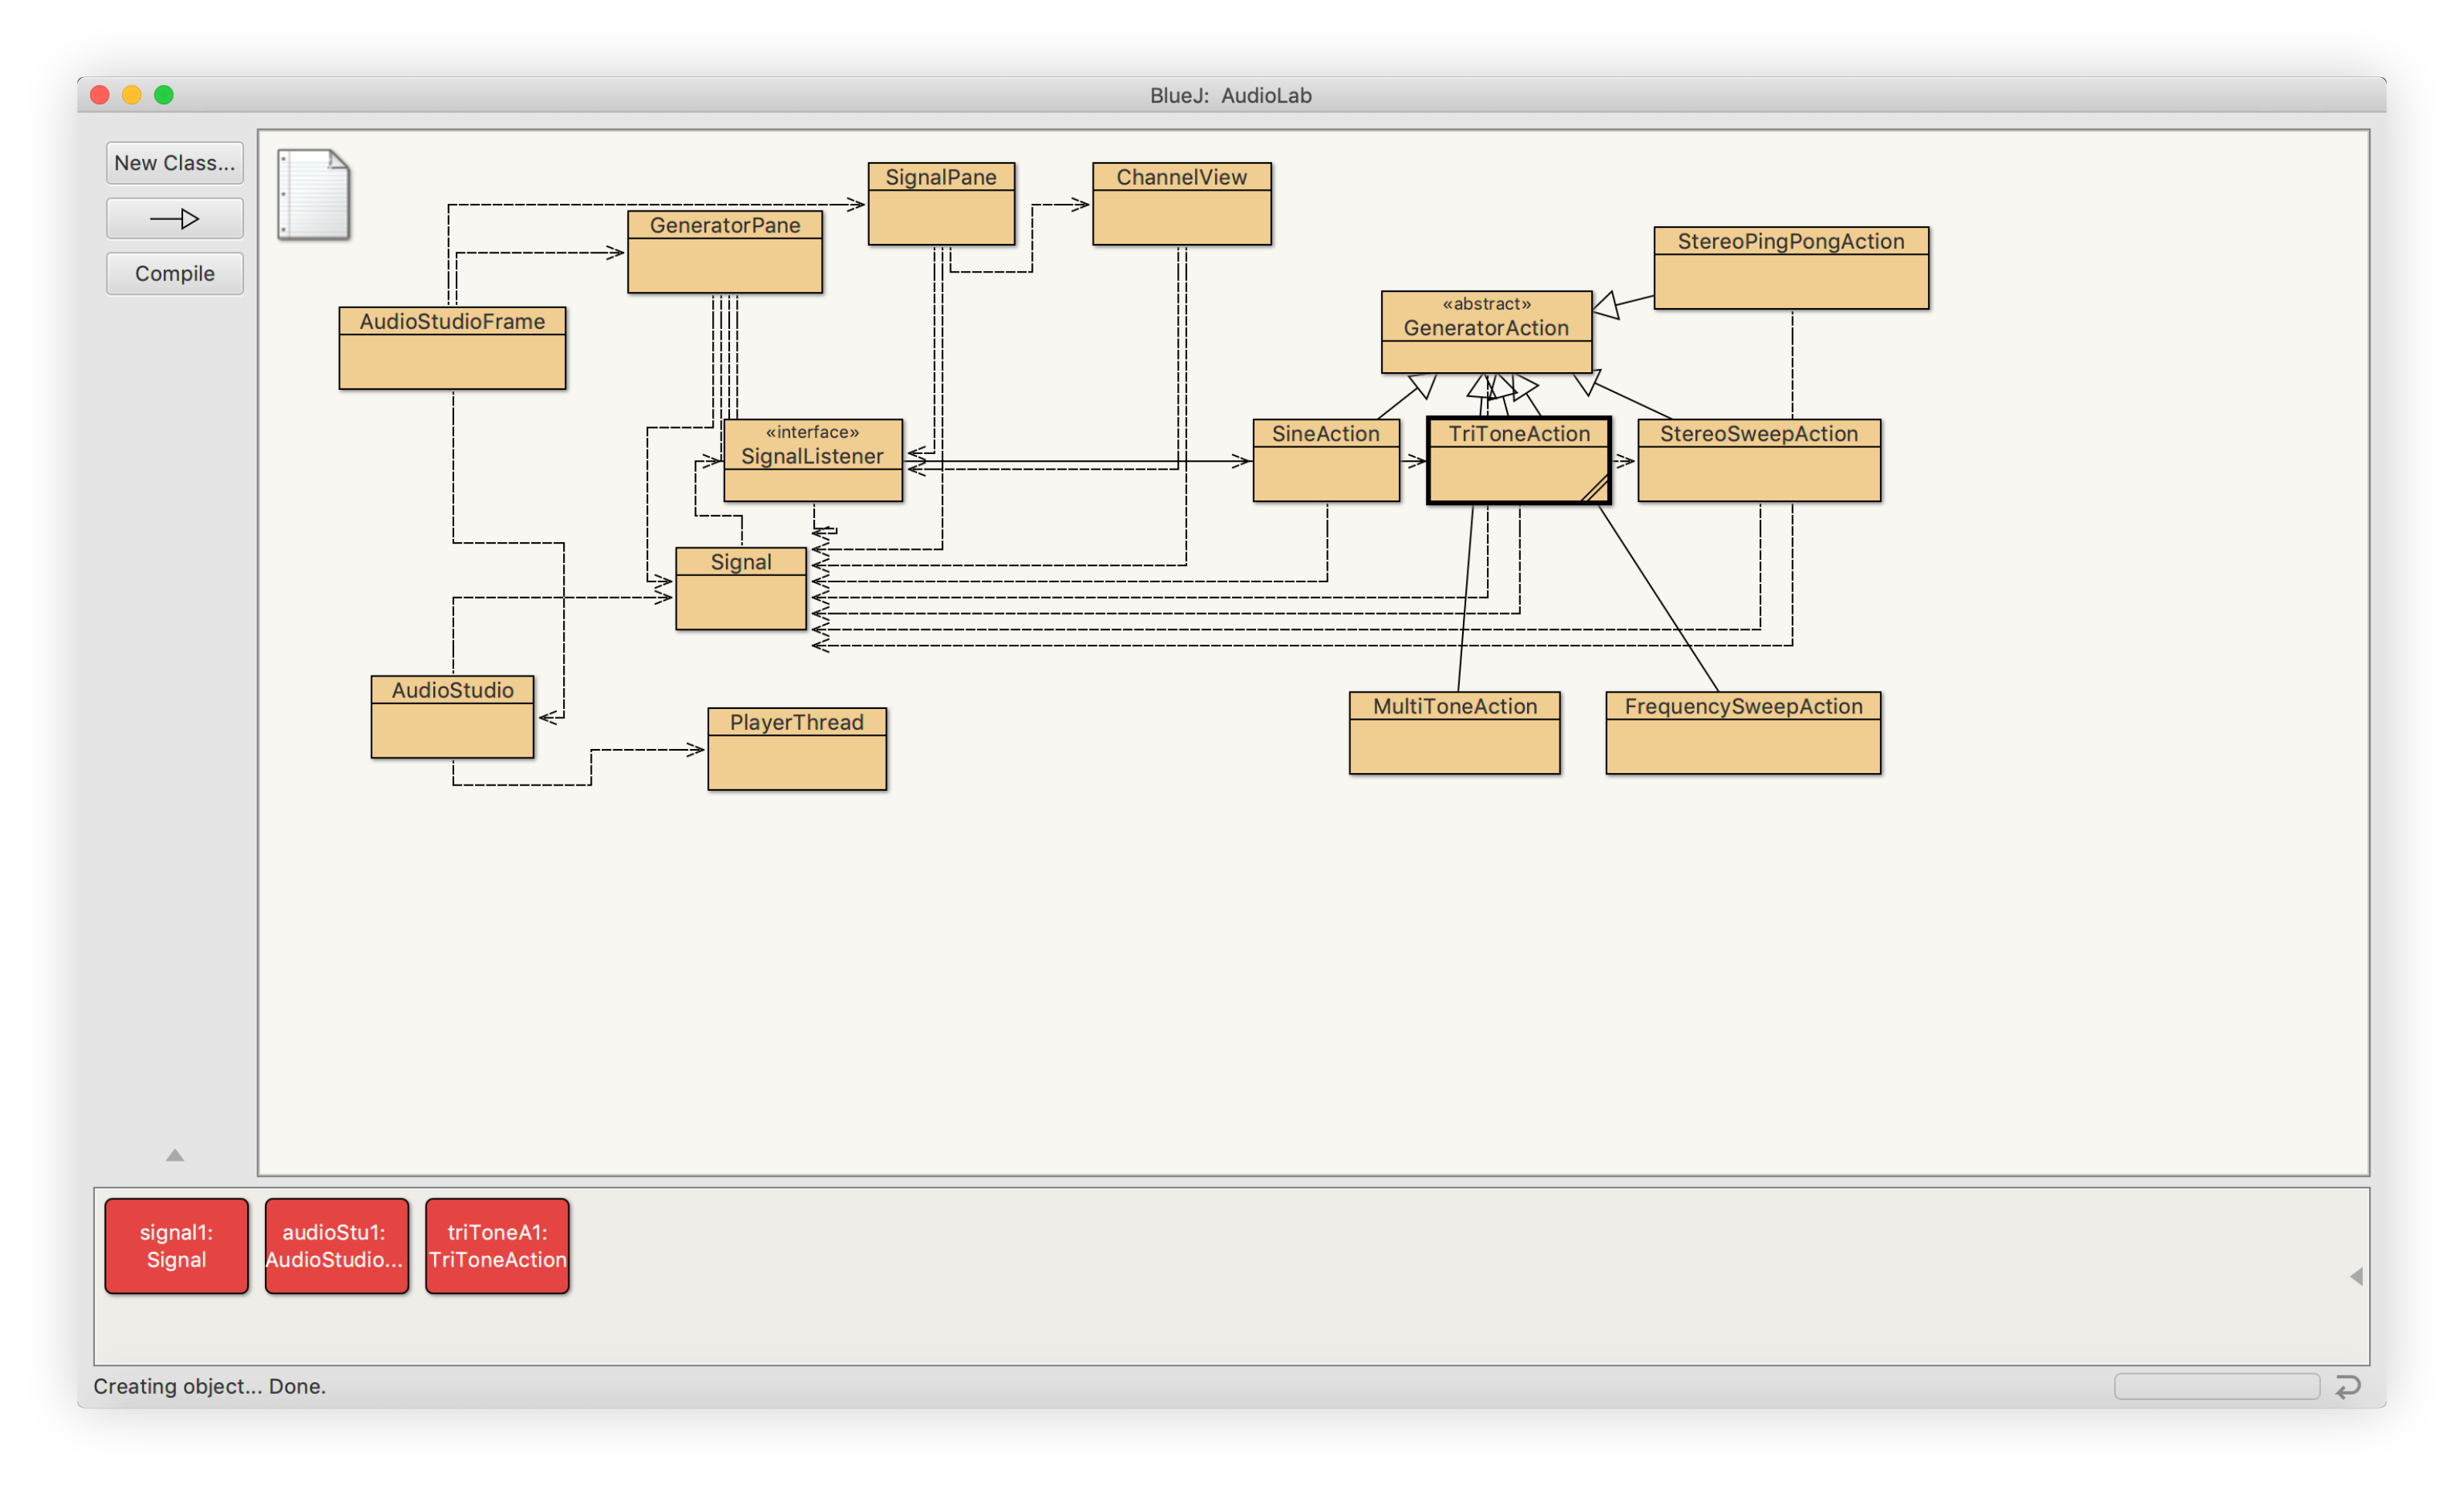
\includegraphics[width=\textwidth]{figures/bluej_classes_objects.png}
\caption {BlueJ and its main view showing the classes of a project and their interconnections, and the Objects Bench at the bottom, showing all the current classes instances.}
\label {bluej_classes_objects}
\end{figure}

\begin{figure}[h]
\centering
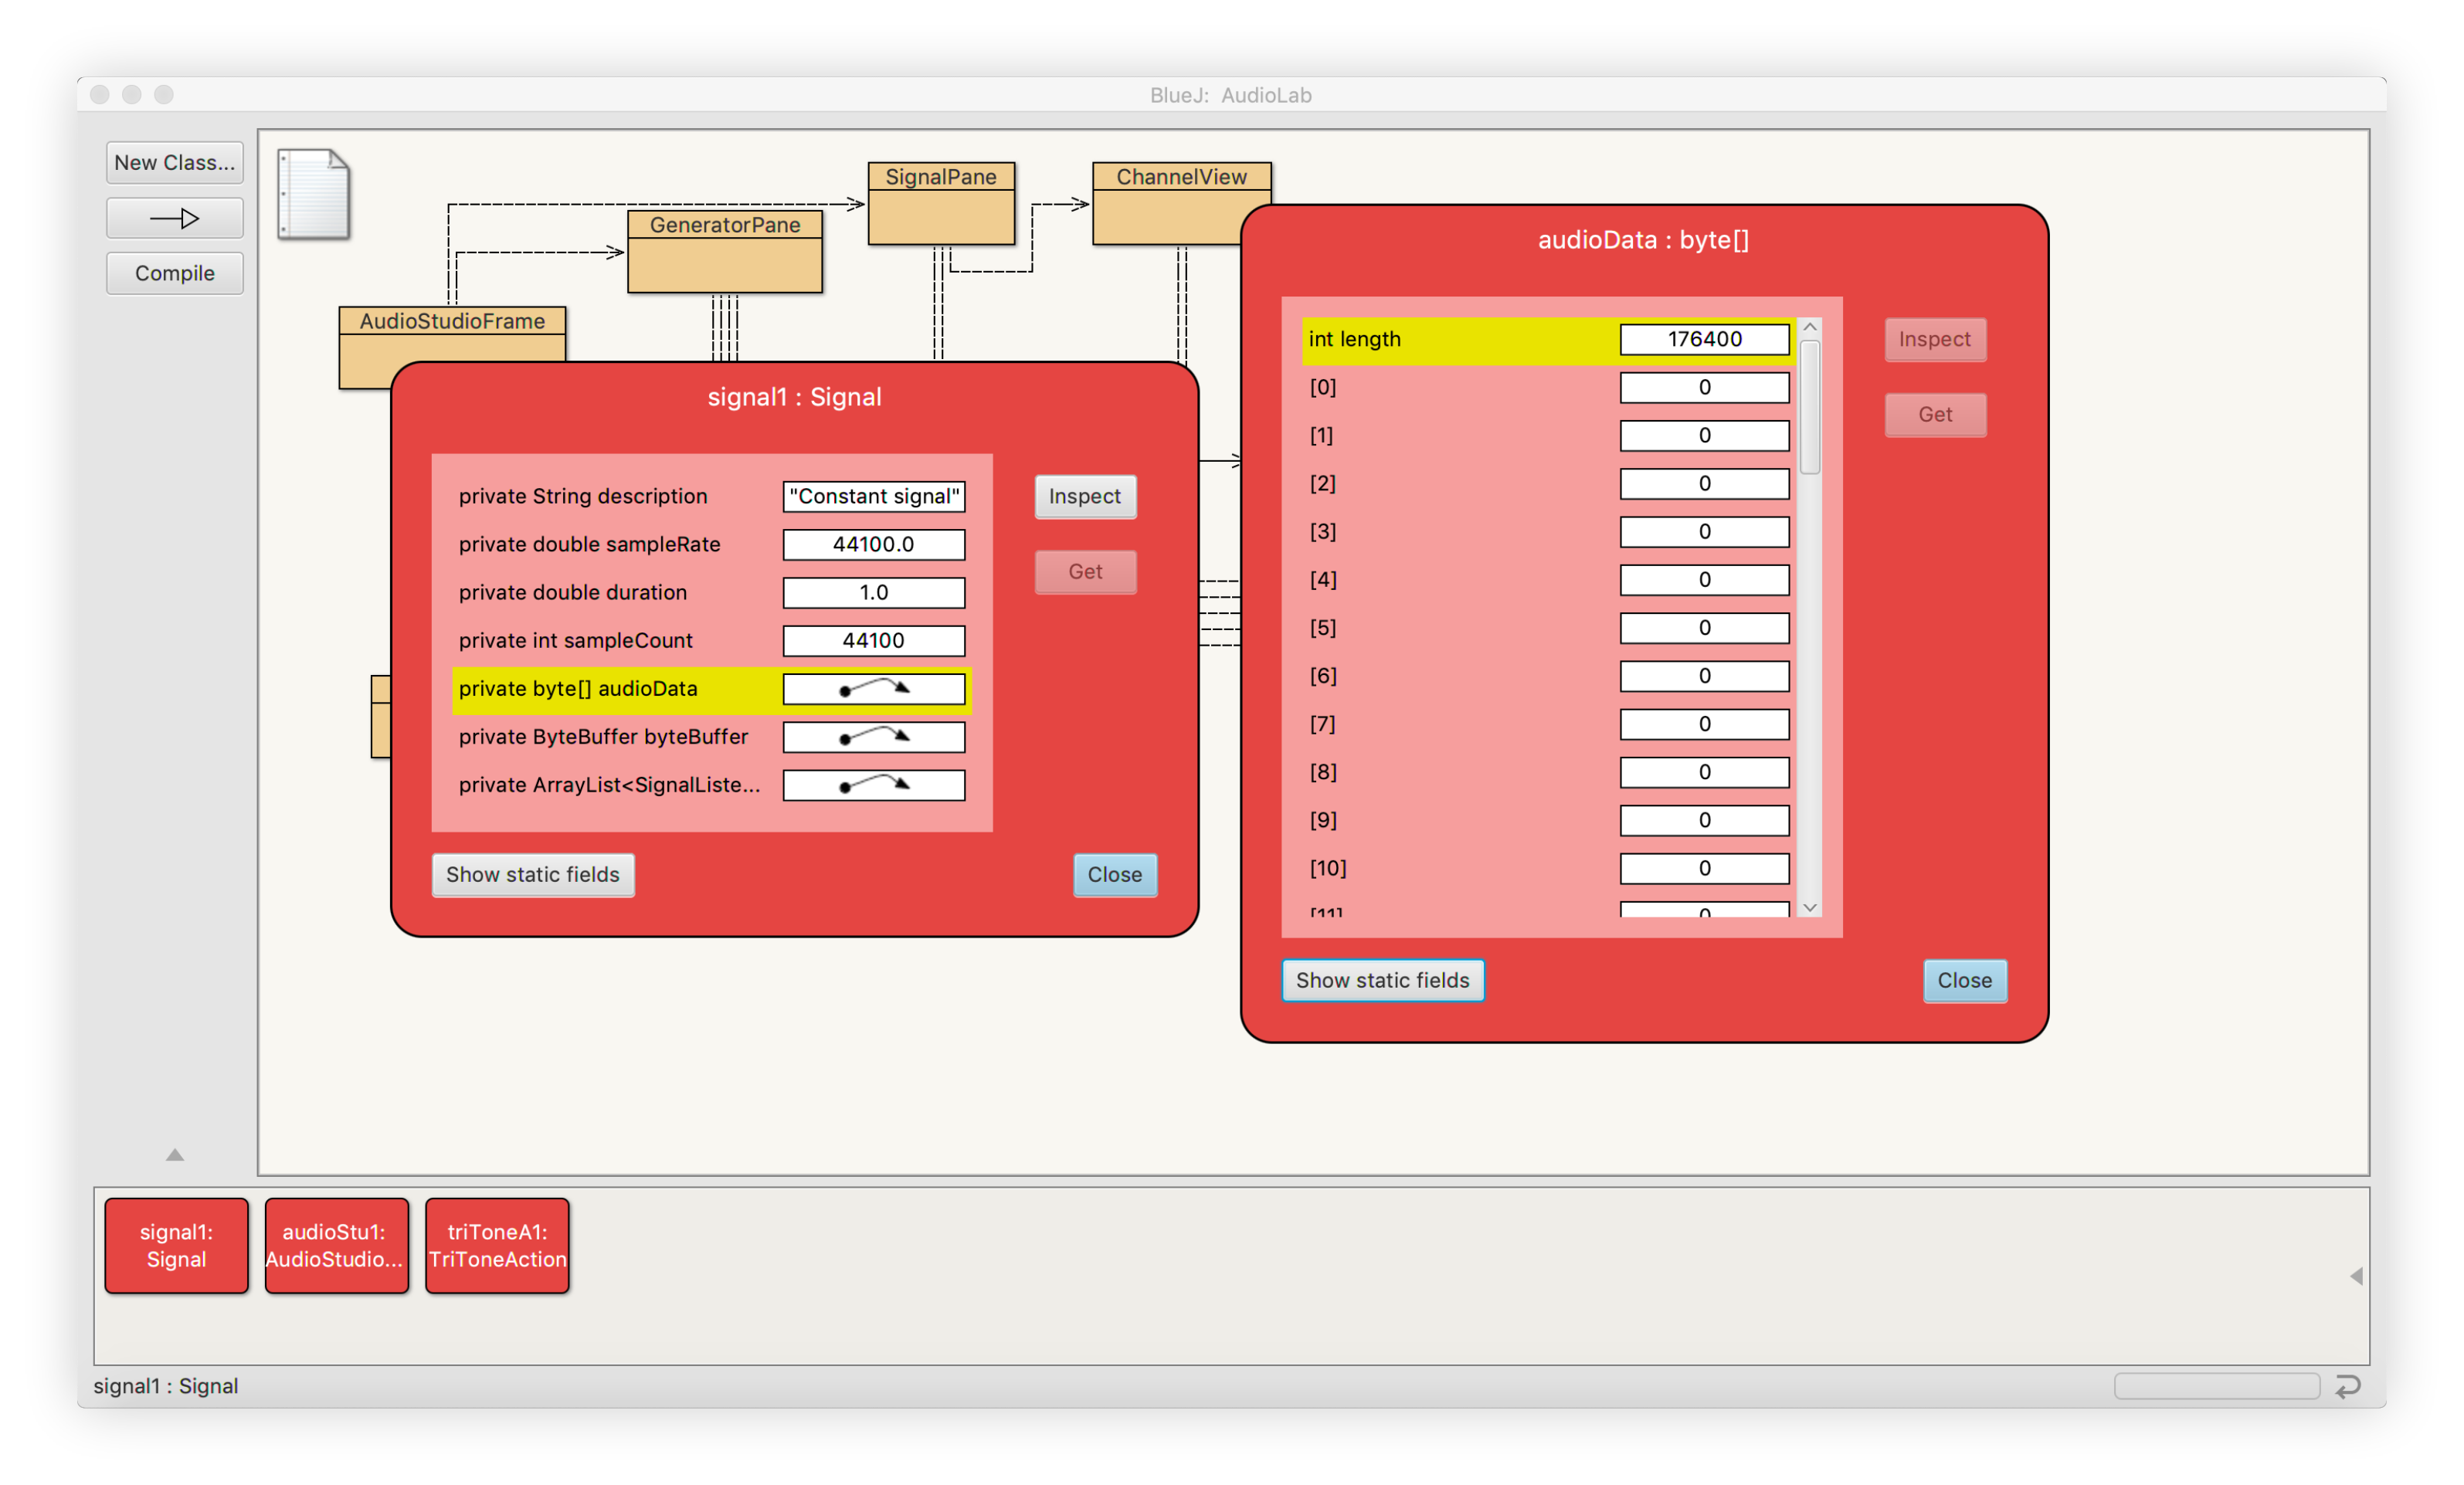
\includegraphics[width=\textwidth]{figures/bluej_objects_open.png}
\caption {Detailed view of an object in BlueJ. As you can see, arrows are only displayed in the main view and for classes. In the object view, reference variable have an arrow icon, which can be double clicked to see what it is referring to.}
\label {bluej_objects_open}
\end{figure}

\subsection{Novis - Michael Berry \& Michael K\"{o}lling}

Novis \cite{7743153} is a notional machine implementation, aimed at beginners and integrated into BlueJ, providing real-time visualisation of the notional machine.

\begin{figure}[h]
\centering
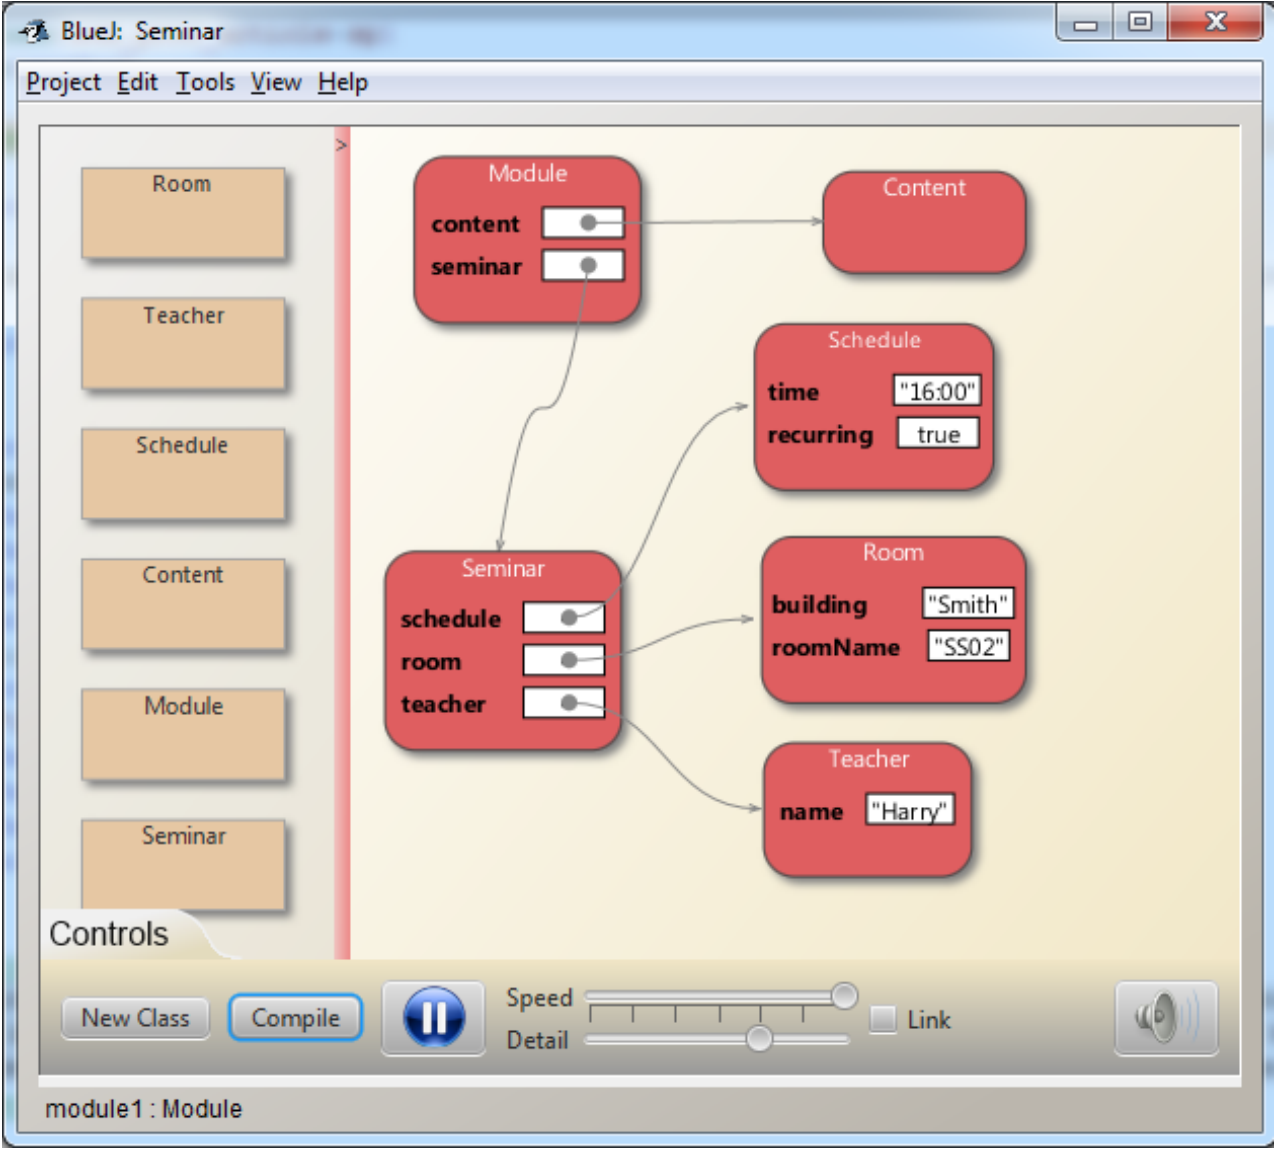
\includegraphics[scale=0.4]{figures/Novis.png}
\caption {Novis.}
\end{figure}

\subsection{JIVE}

JIVE \footnote{\url{https://cse.buffalo.edu/jive/}} stands for \emph{Java Interactive Visualization Environment} and it is an interactive execution for the Eclipse IDE \footnote{\url{https://www.eclipse.org/}} that provides visualizations of Java programs.

\begin{figure}[h]
\centering
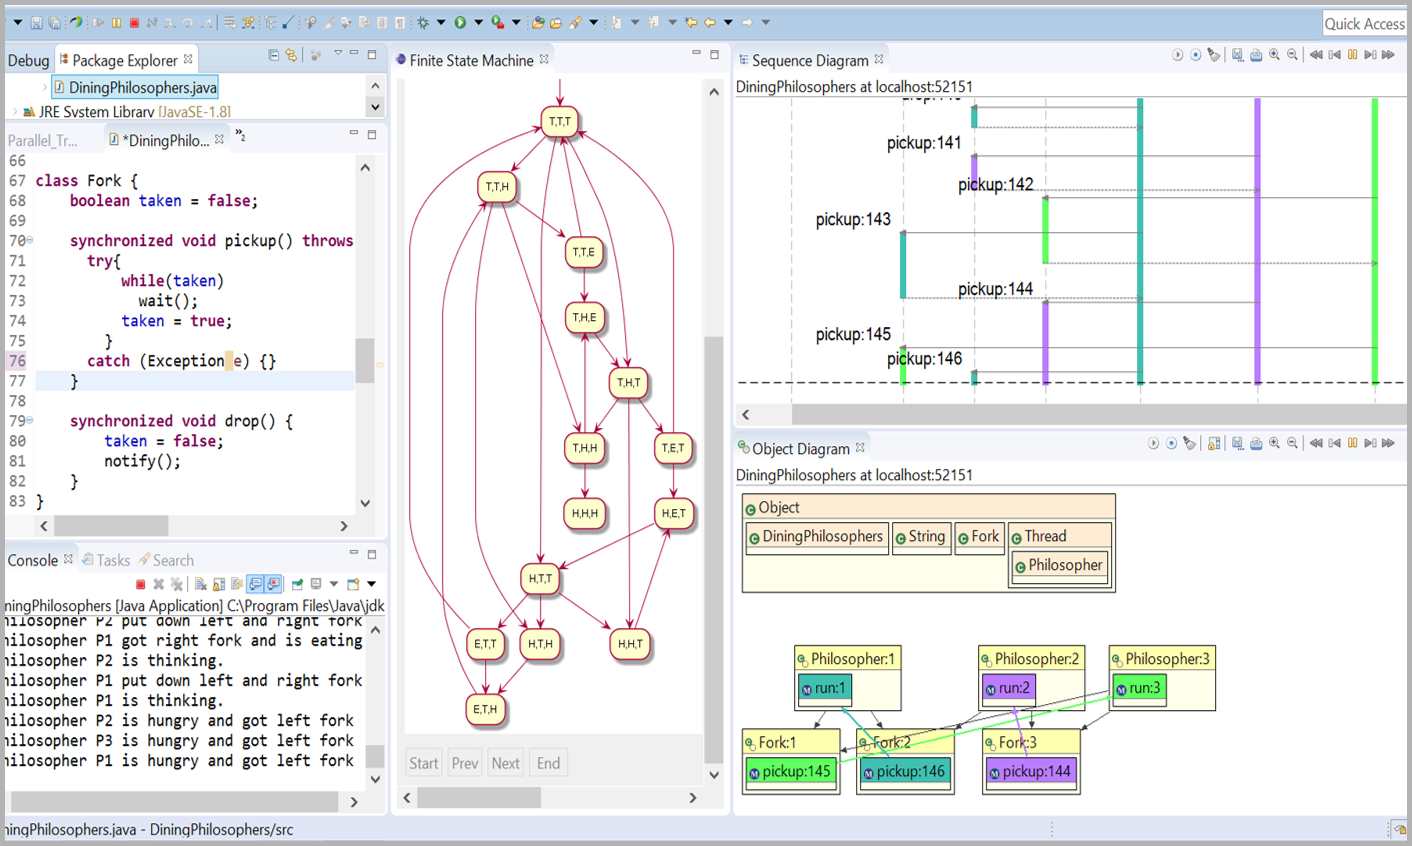
\includegraphics[width=\textwidth]{figures/jive.png}
\caption {JIVE.}
\end{figure}

\subsection{ViLLE}

ViLLE \footnote{\url{https://ville.cs.utu.fi/old/}} is a multi-language program visualization tool developed by the University of Turku in Finland. Like other visualizers, its goal is to support the learning experience of beginner programmers, who might struggle to understand how to code. It has different use cases, for example it can be used to create and edit code snippets and to see in real time what happens during their execution.

\begin{figure}[h]
\centering
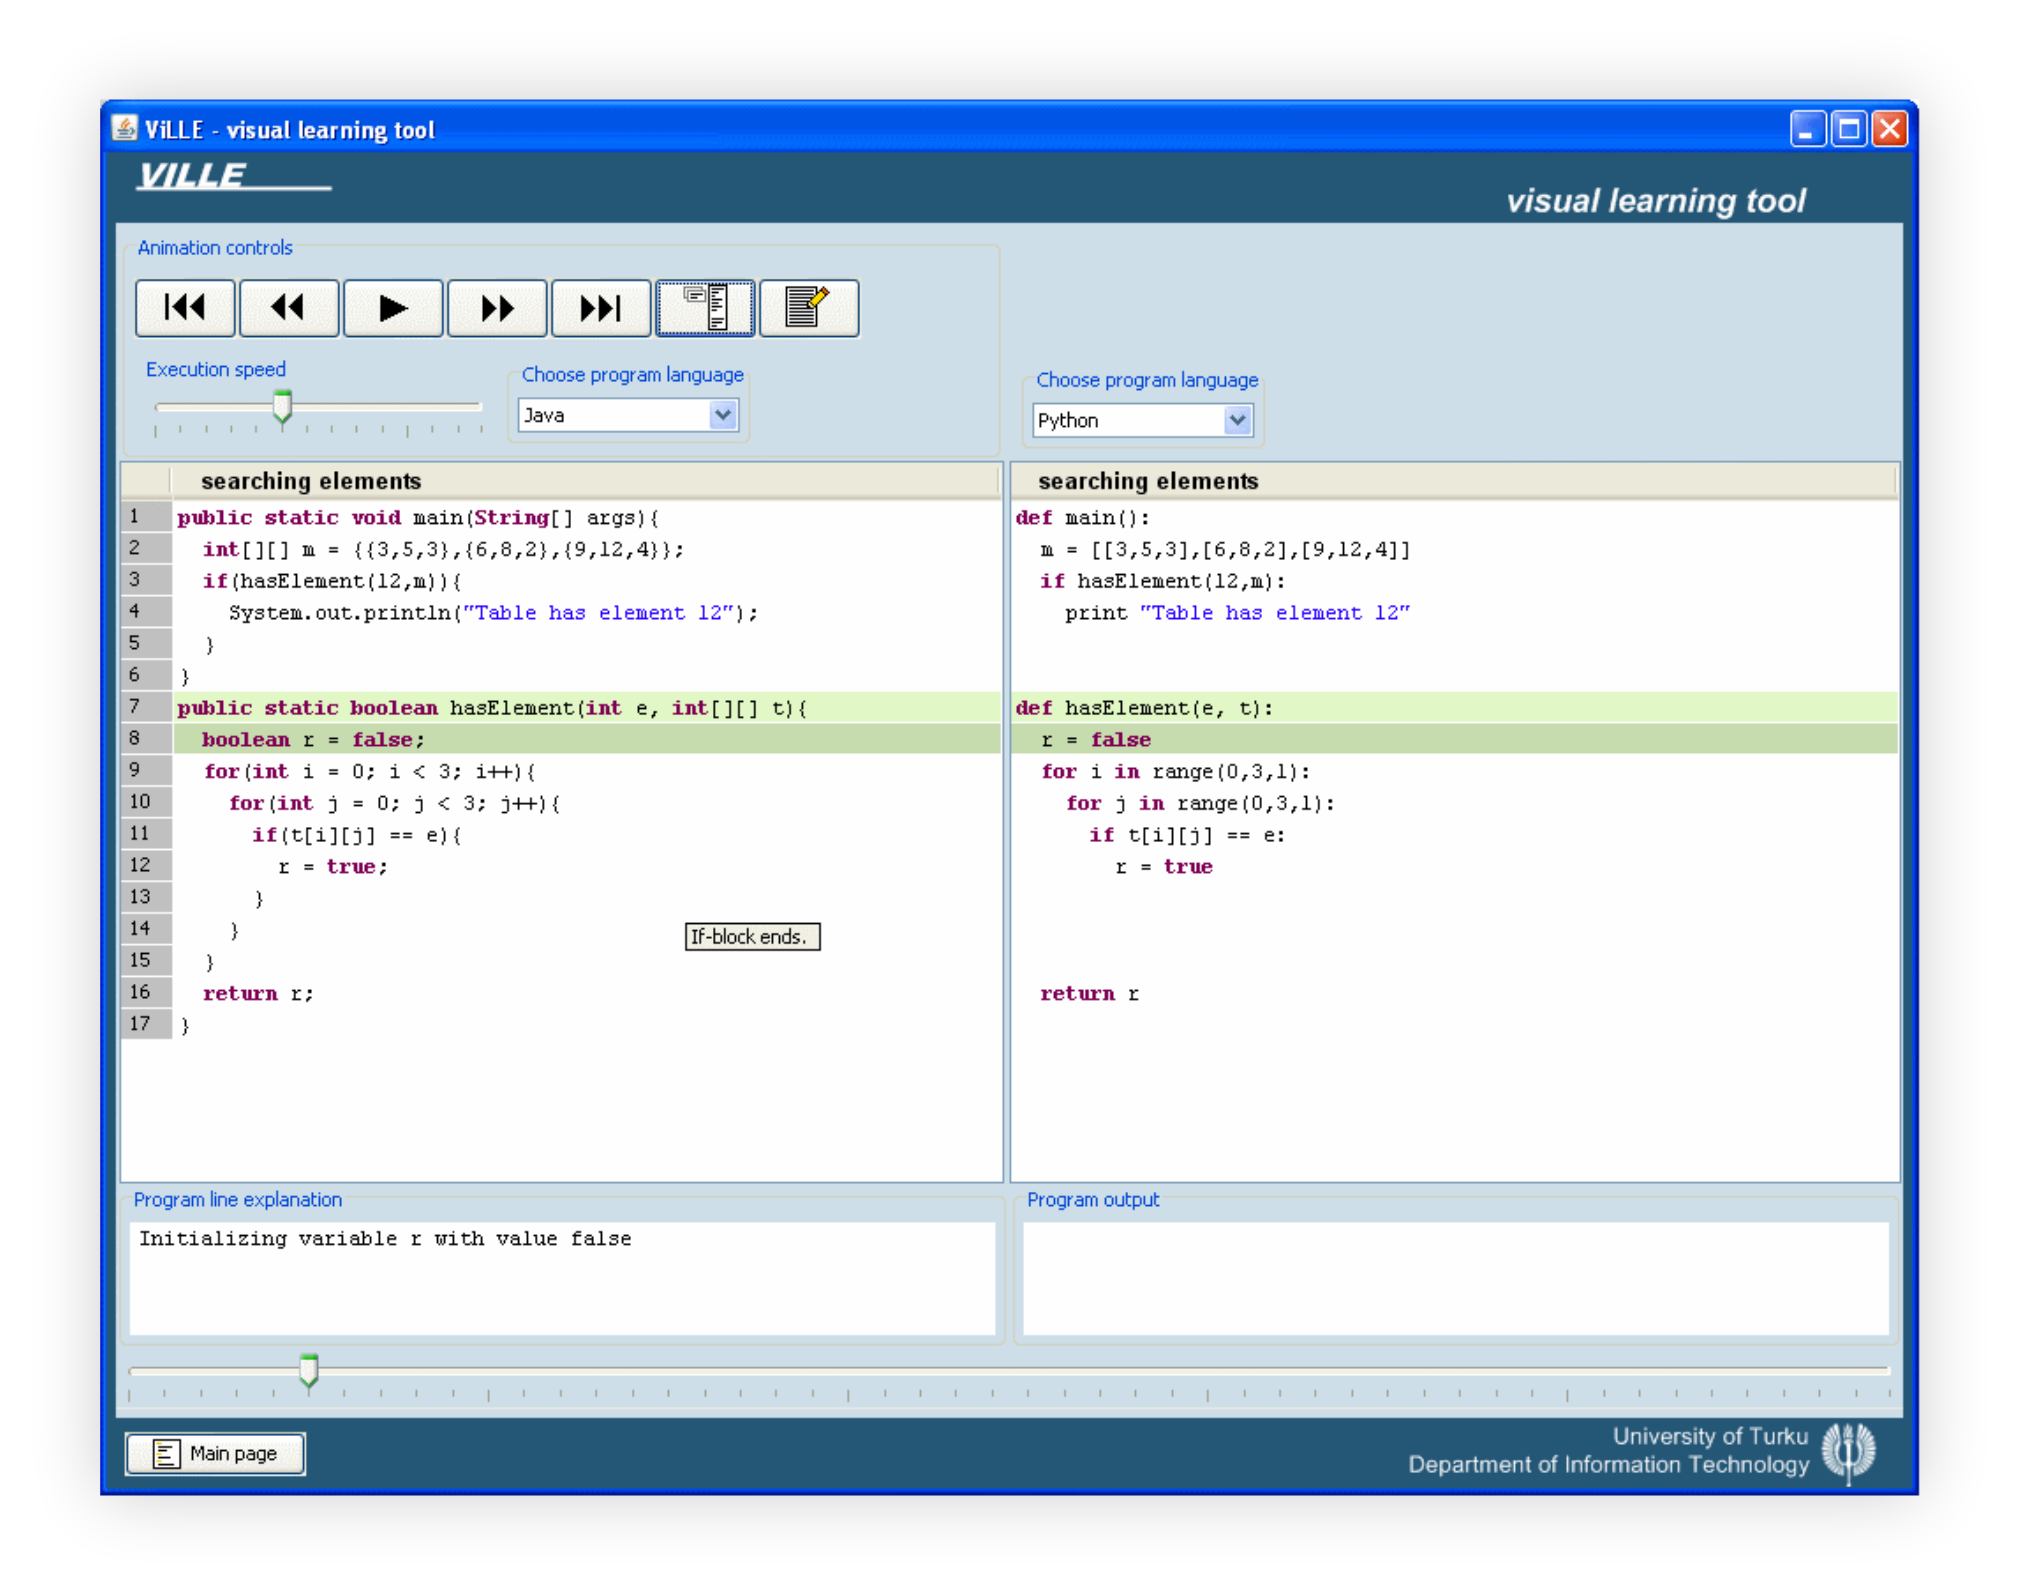
\includegraphics[width=\textwidth]{figures/ville.png}
\caption {ViLLE.}
\end{figure}

\subsection{Python Tutor}

Python Tutor \footnote{\url{http://www.pythontutor.com/}} is a web application for writing some code, see it visualized and executing step by step, and get live help from other users currently on the website.

\begin{figure}[h]
\centering
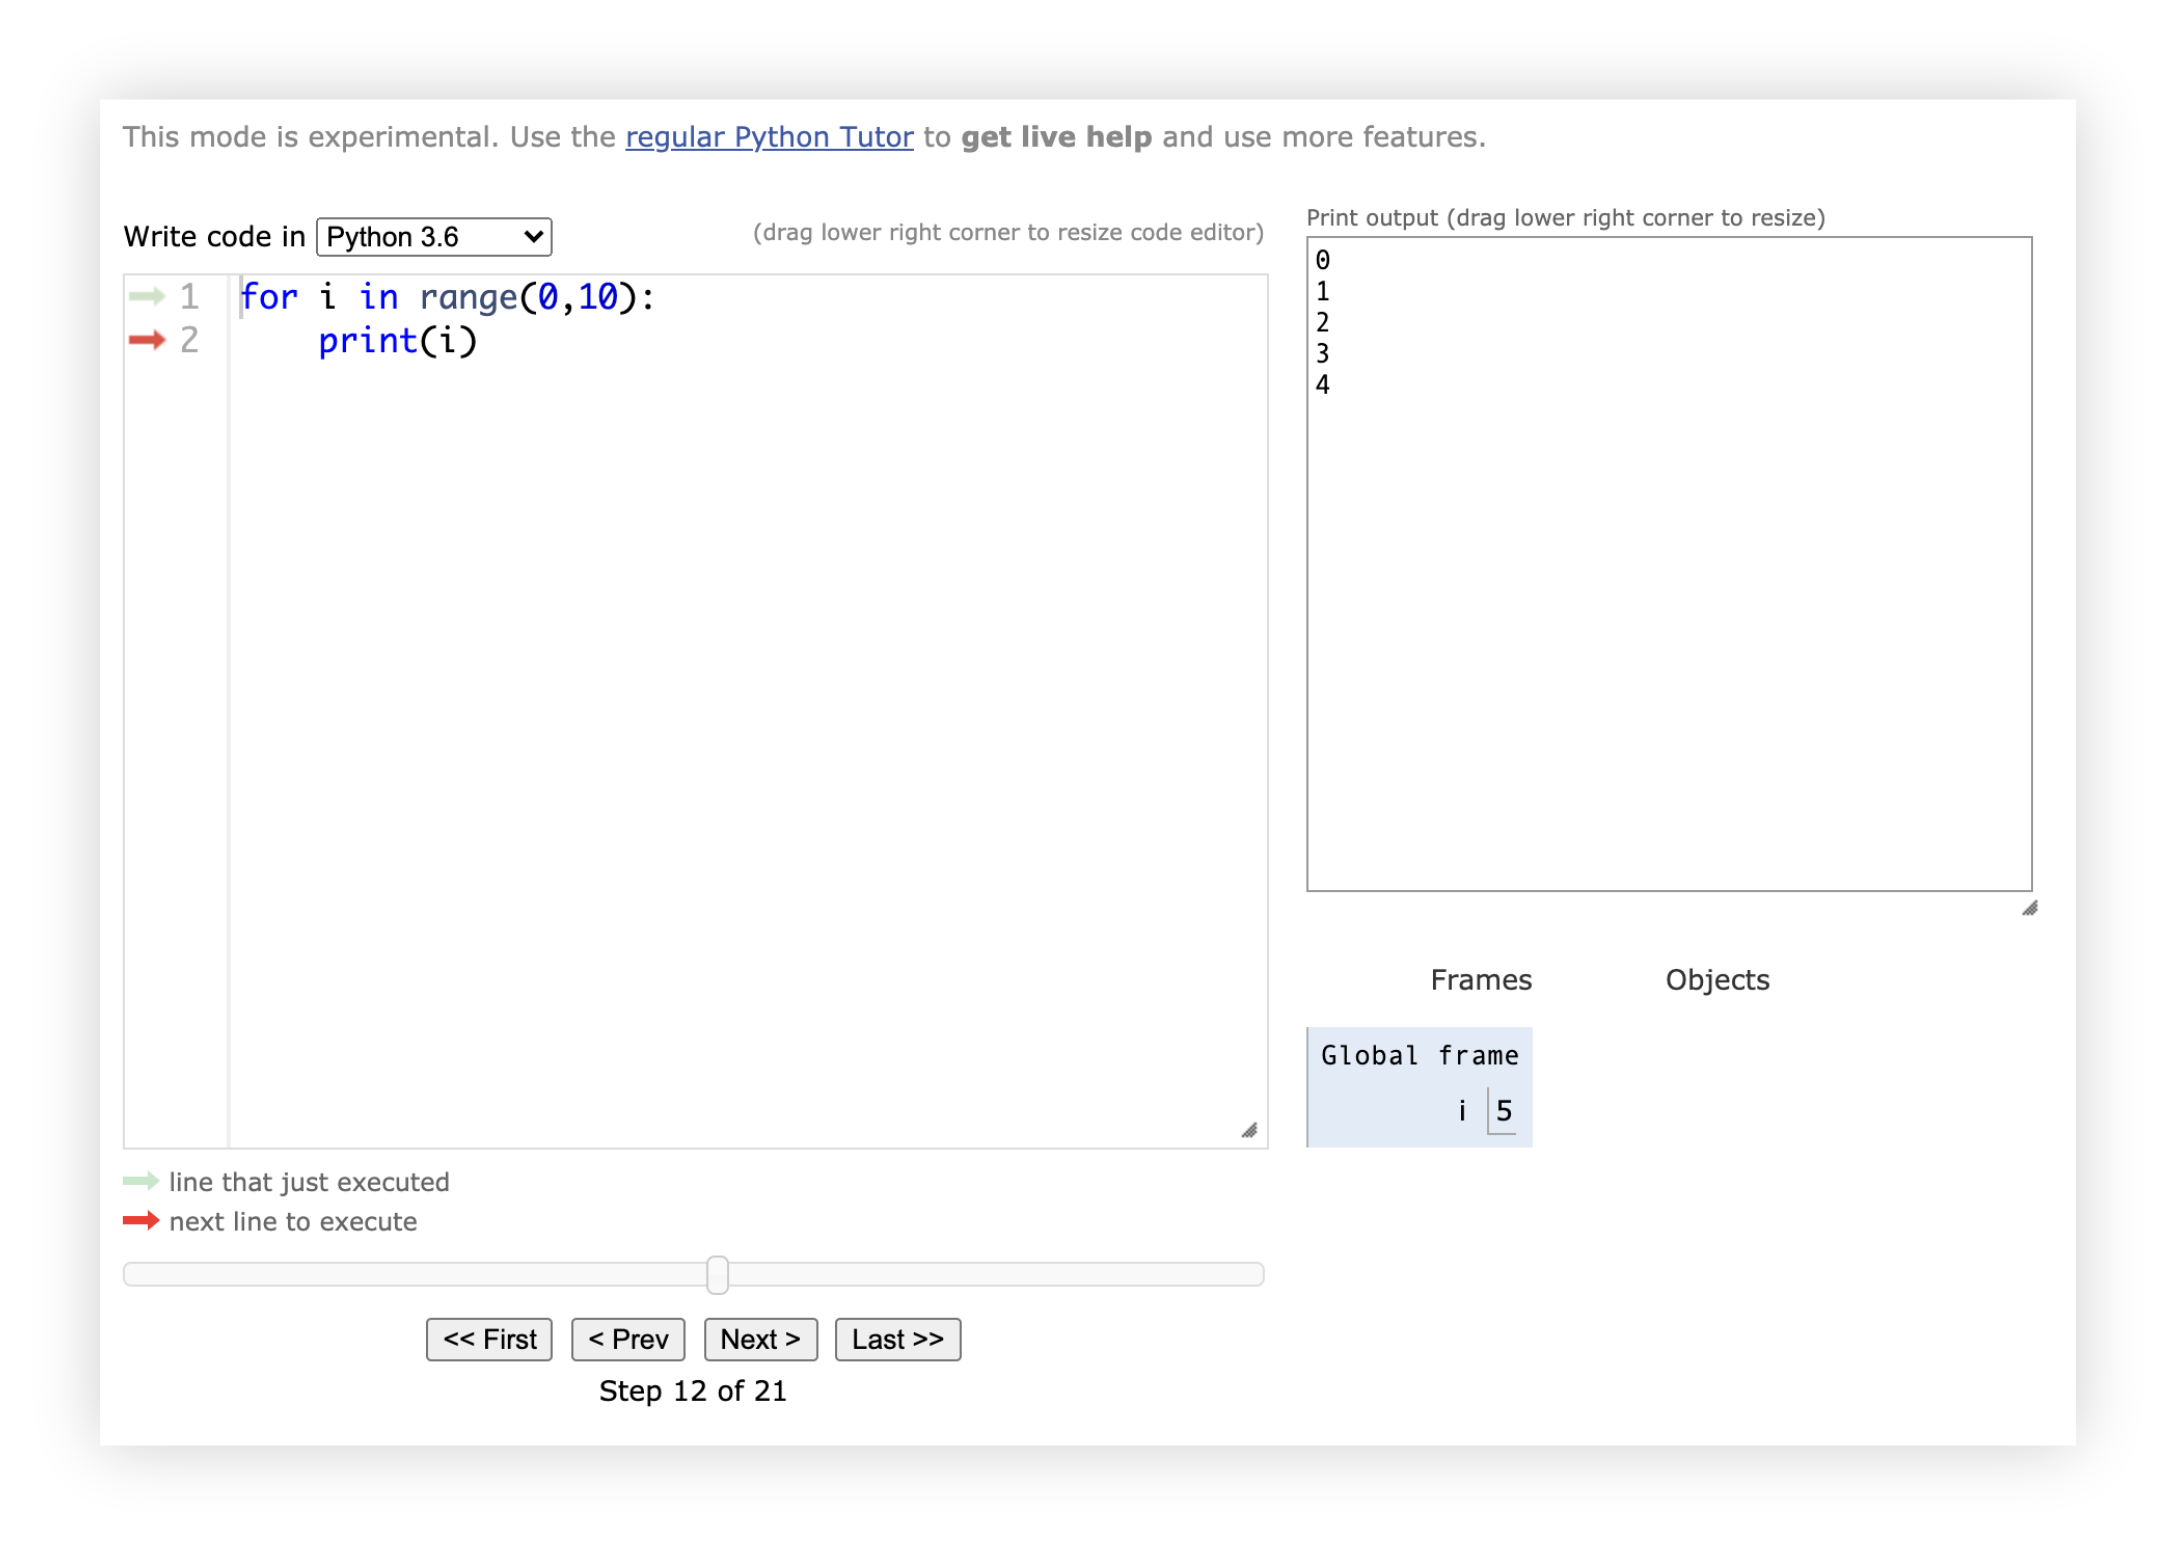
\includegraphics[width=\textwidth]{figures/python_tutor}
\caption {Python tutor.}
\end{figure}

%%%%%%%%%%%%%%%%%%%%%%%%%
\section{Project analysis and requirements} \label{requirements+analysis}
%%%%%%%%%%%%%%%%%%%%%%%%%

In this section I am going to talk about the pre-production phase of the project, from the UI/UX analysis of the main Informa clicker tool, to the basic requirements that were decided as a baseline for the project.

\subsection{UI/UX analysis}

As already mentioned in \hyperref[goal]{\textbf{Section 1.3}}, the main goal of this project was to create an improved and web-based version of the already existing Stack and Heap Diagrams in the Informa clicker tool. In order to understand what worked and what did not work, I did an analysis of its user interface (UI) and user experience (UX) and here is what I found:\\

\textbf{\ul{UI - What works:}}

\begin{itemize}
	\item Arrows always point to the center of the target block, avoiding arrows overlapping.
	\item The interface has a good layout, as all elements are properly positioned following a clear and organized structure.
\end{itemize}\

\textbf{\ul{UI - What does not work:}}

\begin{itemize}
	\item Not enough overall white space \footnote{\url{https://blog.bannersnack.com/white-space-in-graphic-design/}}.
	\item Colors can be improved, because they do not convey a lot of excitement being very pale. In this case, saturation be help create a more engaging experience.
	\item All buttons that appear on mouseover events substantially clutter the interface and hide too many elements.
	\item Space dedicated to the diagram is relatively small compared to the whole screen.
	\item The buttons in the top toolbar are not styled as buttons.
\end{itemize}\

\textbf{\ul{UX - What works:}}

\begin{itemize}
	\item The interface is generally very intuitive thanks to its already praised layout, and I did not have any issues pursuing any task.
\end{itemize}\

\textbf{\ul{UX - What does not work:}}

\begin{itemize}
	\item The buttons at the top of the diagram, by not looking like buttons, make their purpose unclear to the user.
	\item Dragging the start of an arrow starting from a stack frame, makes it snap back to the border of a given block instead of the center of a variable.
\end{itemize}\

\noindent As you can read from this analysis, the result is pretty clear: the Informa clicker does not have any problem in terms of user experience, but it lacks a proper user interface to better deliver what already works.

\subsection{Requirements}

After running the UI/UX analysis and establishing that what had to be improved was the UI, prof. Hauswirth and I set as minimum requirements all the features the clicker already has. In particular users can:

\begin{enumerate}
	\item Freely create stack frames and heap objects by dragging and dropping them onto the interface.
	\item Add and remove primitive and reference/instance variables from a given block \footnote{A block is a general term for stack frames and heap objects.}.
	\item Create arrows by clicking on a reference variable, holding that click and releasing it on a heap object.
	\item Drag blocks around.
\end{enumerate}

\pagebreak
\vspace{\fill}

\noindent Plus something new:

\begin{enumerate}
	\item A data structure must be updated with every state change within within the diagram (more on this is \hyperref[storing states]{\textbf{Section 4.4}}), and eventually be converted to a JSON file more offline editing and automating tests on Informa.
	\item Clear division between stack and heap.
\end{enumerate}

\subsection{Extra features}

Alongside the requirements, we have also agreed upon a set of possible bonus features that could be added if I would have finished the project early:

\begin{enumerate}
	\item The JSON file which represents the current state of the diagram, can both be downloaded and uploaded into the web application. Uploading that file acts like loading a save state in a videogame, because the whole interface goes back as it was left at the time of downloading the JSON file.
	\item Panning and zooming around in the interface.
	\item Arrows as polygonal chains \footnote{\url{https://en.wikipedia.org/wiki/Polygonal_chain}}.
\end{enumerate}

\vspace{\fill}

\pagebreak

%%%%%%%%%%%%%%%%%%%%%%%%%
\section{Project design} \label{design}
%%%%%%%%%%%%%%%%%%%%%%%%%

In this section I am going to describe the design process, not only coding-wise but also from the graphics perspective, elaborating all the decisions and solutions I had to make during this critical development phase. The design process can, in fact, either make or break the entire project. Making awful decisions at this stage, causes unavoidable problems down the line and it is the precise reason why I took maybe a bit more time than what I had initially planned, and only start coding when we were satisfied enough with the result.

\subsection{UI/UX research} \label{ui-ux research}

In \hyperref[requirements+analysis]{\textbf{Section 3}}, we saw how the biggest problem of the Informa clicker tool was the user interface and because of that, the first week and a half were completely spent sketching ideas on paper, bringing the best ones in Figma \footnote{My go-to UI/UX design editor (\url{https://www.figma.com/}).} and ultimately creating the high-fidelity mockups \footnote{Full size model of a design or device, used for product presentations or other purposes.} to show to prof. Hauswirth in order to get feedback.\\
The first step was to figure out how to divide the stack and heap areas, since one of the requirements was about having a clear distinction between the two. In my mind there were two possible ways to approach this: either using a floating or docked stack.\\

\noindent \hyperref[floating stack]{\textbf{Figure 7}} shows the first version of the user interface with a floating stack, and even though it is indeed separate from the heap and it might look somewhat cool, I did not like the clunkiness of having such an imposing object in the scene. However, one important solution was carried on until the end of the project, and that was the block data encapsulation, a fancy expression to indicate that every object has all its information contained within a rectangular shape. The Informa clicker is very similar in this regard, since it has all variables in a similar looking element, so it is not a big change, but it certainly helps "glueing" the data and offers clearer separation between blocks.\\
As far as stack frames and heap objects, I tried to adopt a more schematic approach, and reserve one row for each detail (name, type and value) of every variable. However, this idea was eventually dropped because it took up too much space, and the number of variables that were visible without causing the stack content to be scrollable, was extremely low. 

\begin{figure}[h!]
\centering
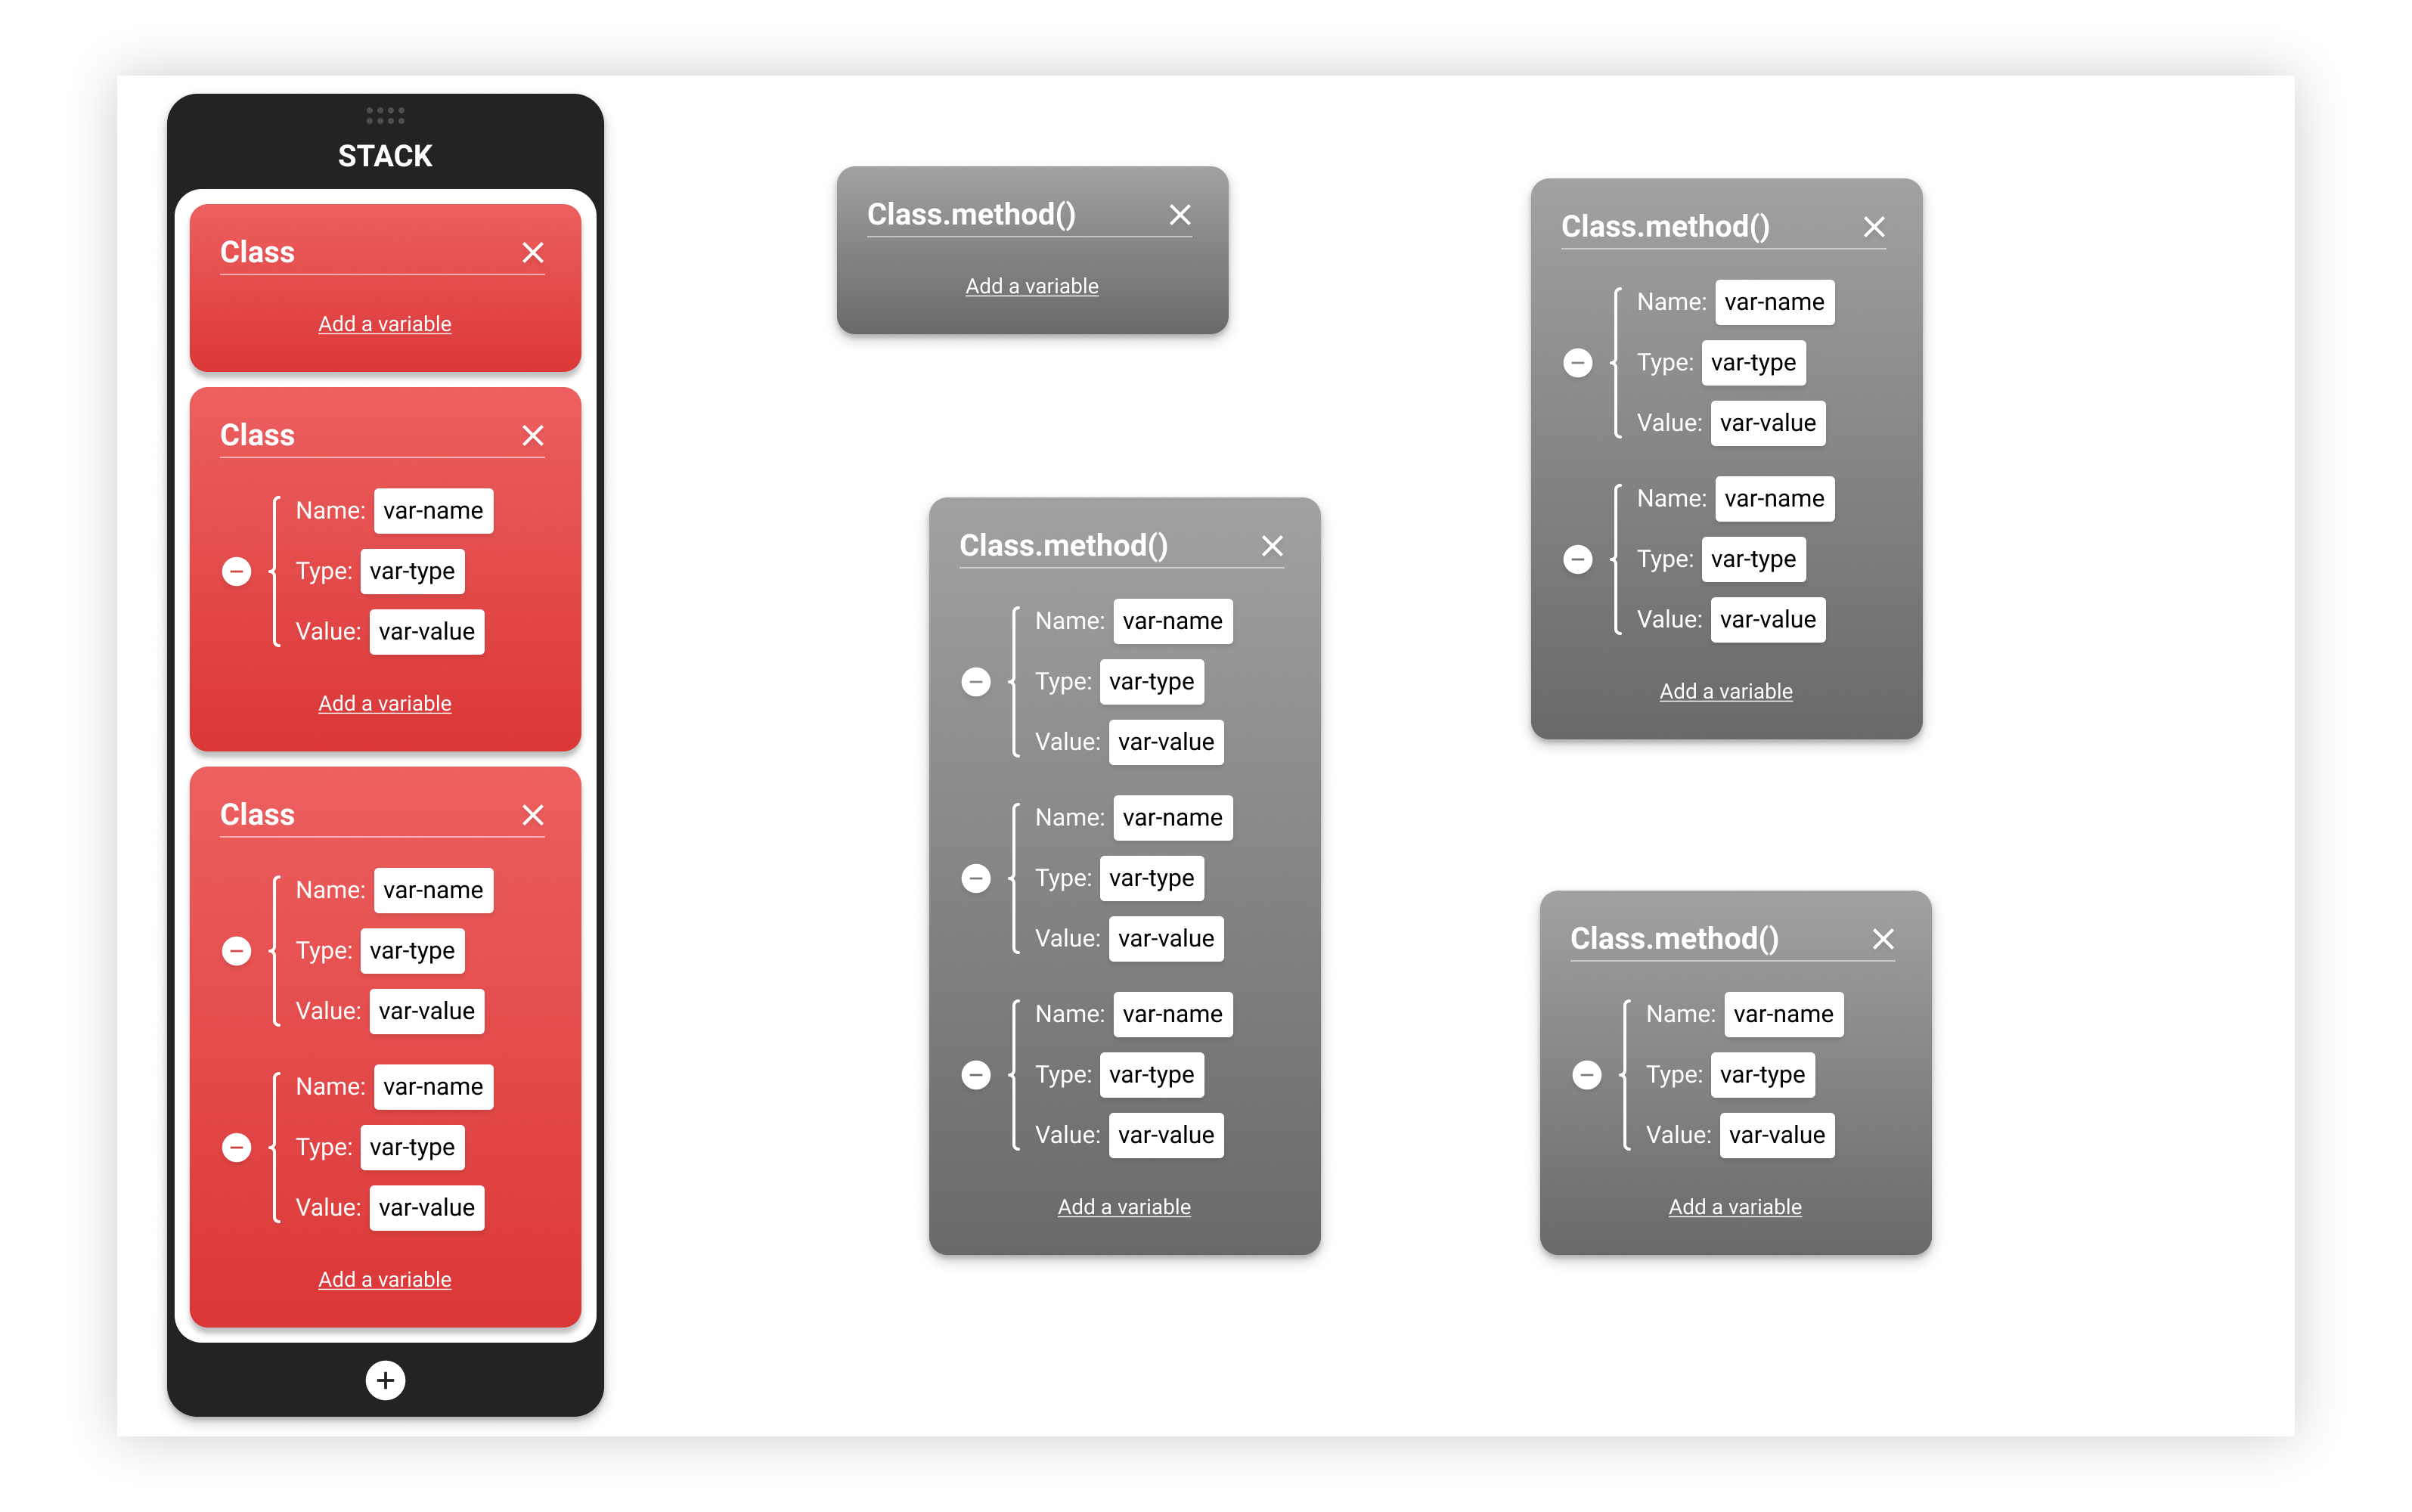
\includegraphics[width=\textwidth]{figures/floating_stack.png}
\caption {First version of the user interface, with a floating stack}
\label{floating stack}
\end{figure}

\pagebreak

\noindent \hyperref[separate regions]{\textbf{Figure 8}} shows an intermediate version of the design, which is substantially different from the previous one shown in \hyperref[floating stack]{\textbf{Figure 7}}. In fact, I tried to develop the idea of a docked stack. Actually, if compared to having it floating it might even have a few disadvantages, such as the impossibility of moving it around and occupying a fixed amount of space, which will not be available to the heap. On the other hand, it is stylistically a lot nicer on the eyes and it definitely delivers the best separation between the two regions. I also started playing with colors, in order to bring out a bit more playfulness from a rather schematic UI.\\
Besides stack and heap being separated by a divider, each has a header which labels the region where the user is working, and a plus button to add new stack frames and new heap objects.

\begin{figure}[h!]
\centering
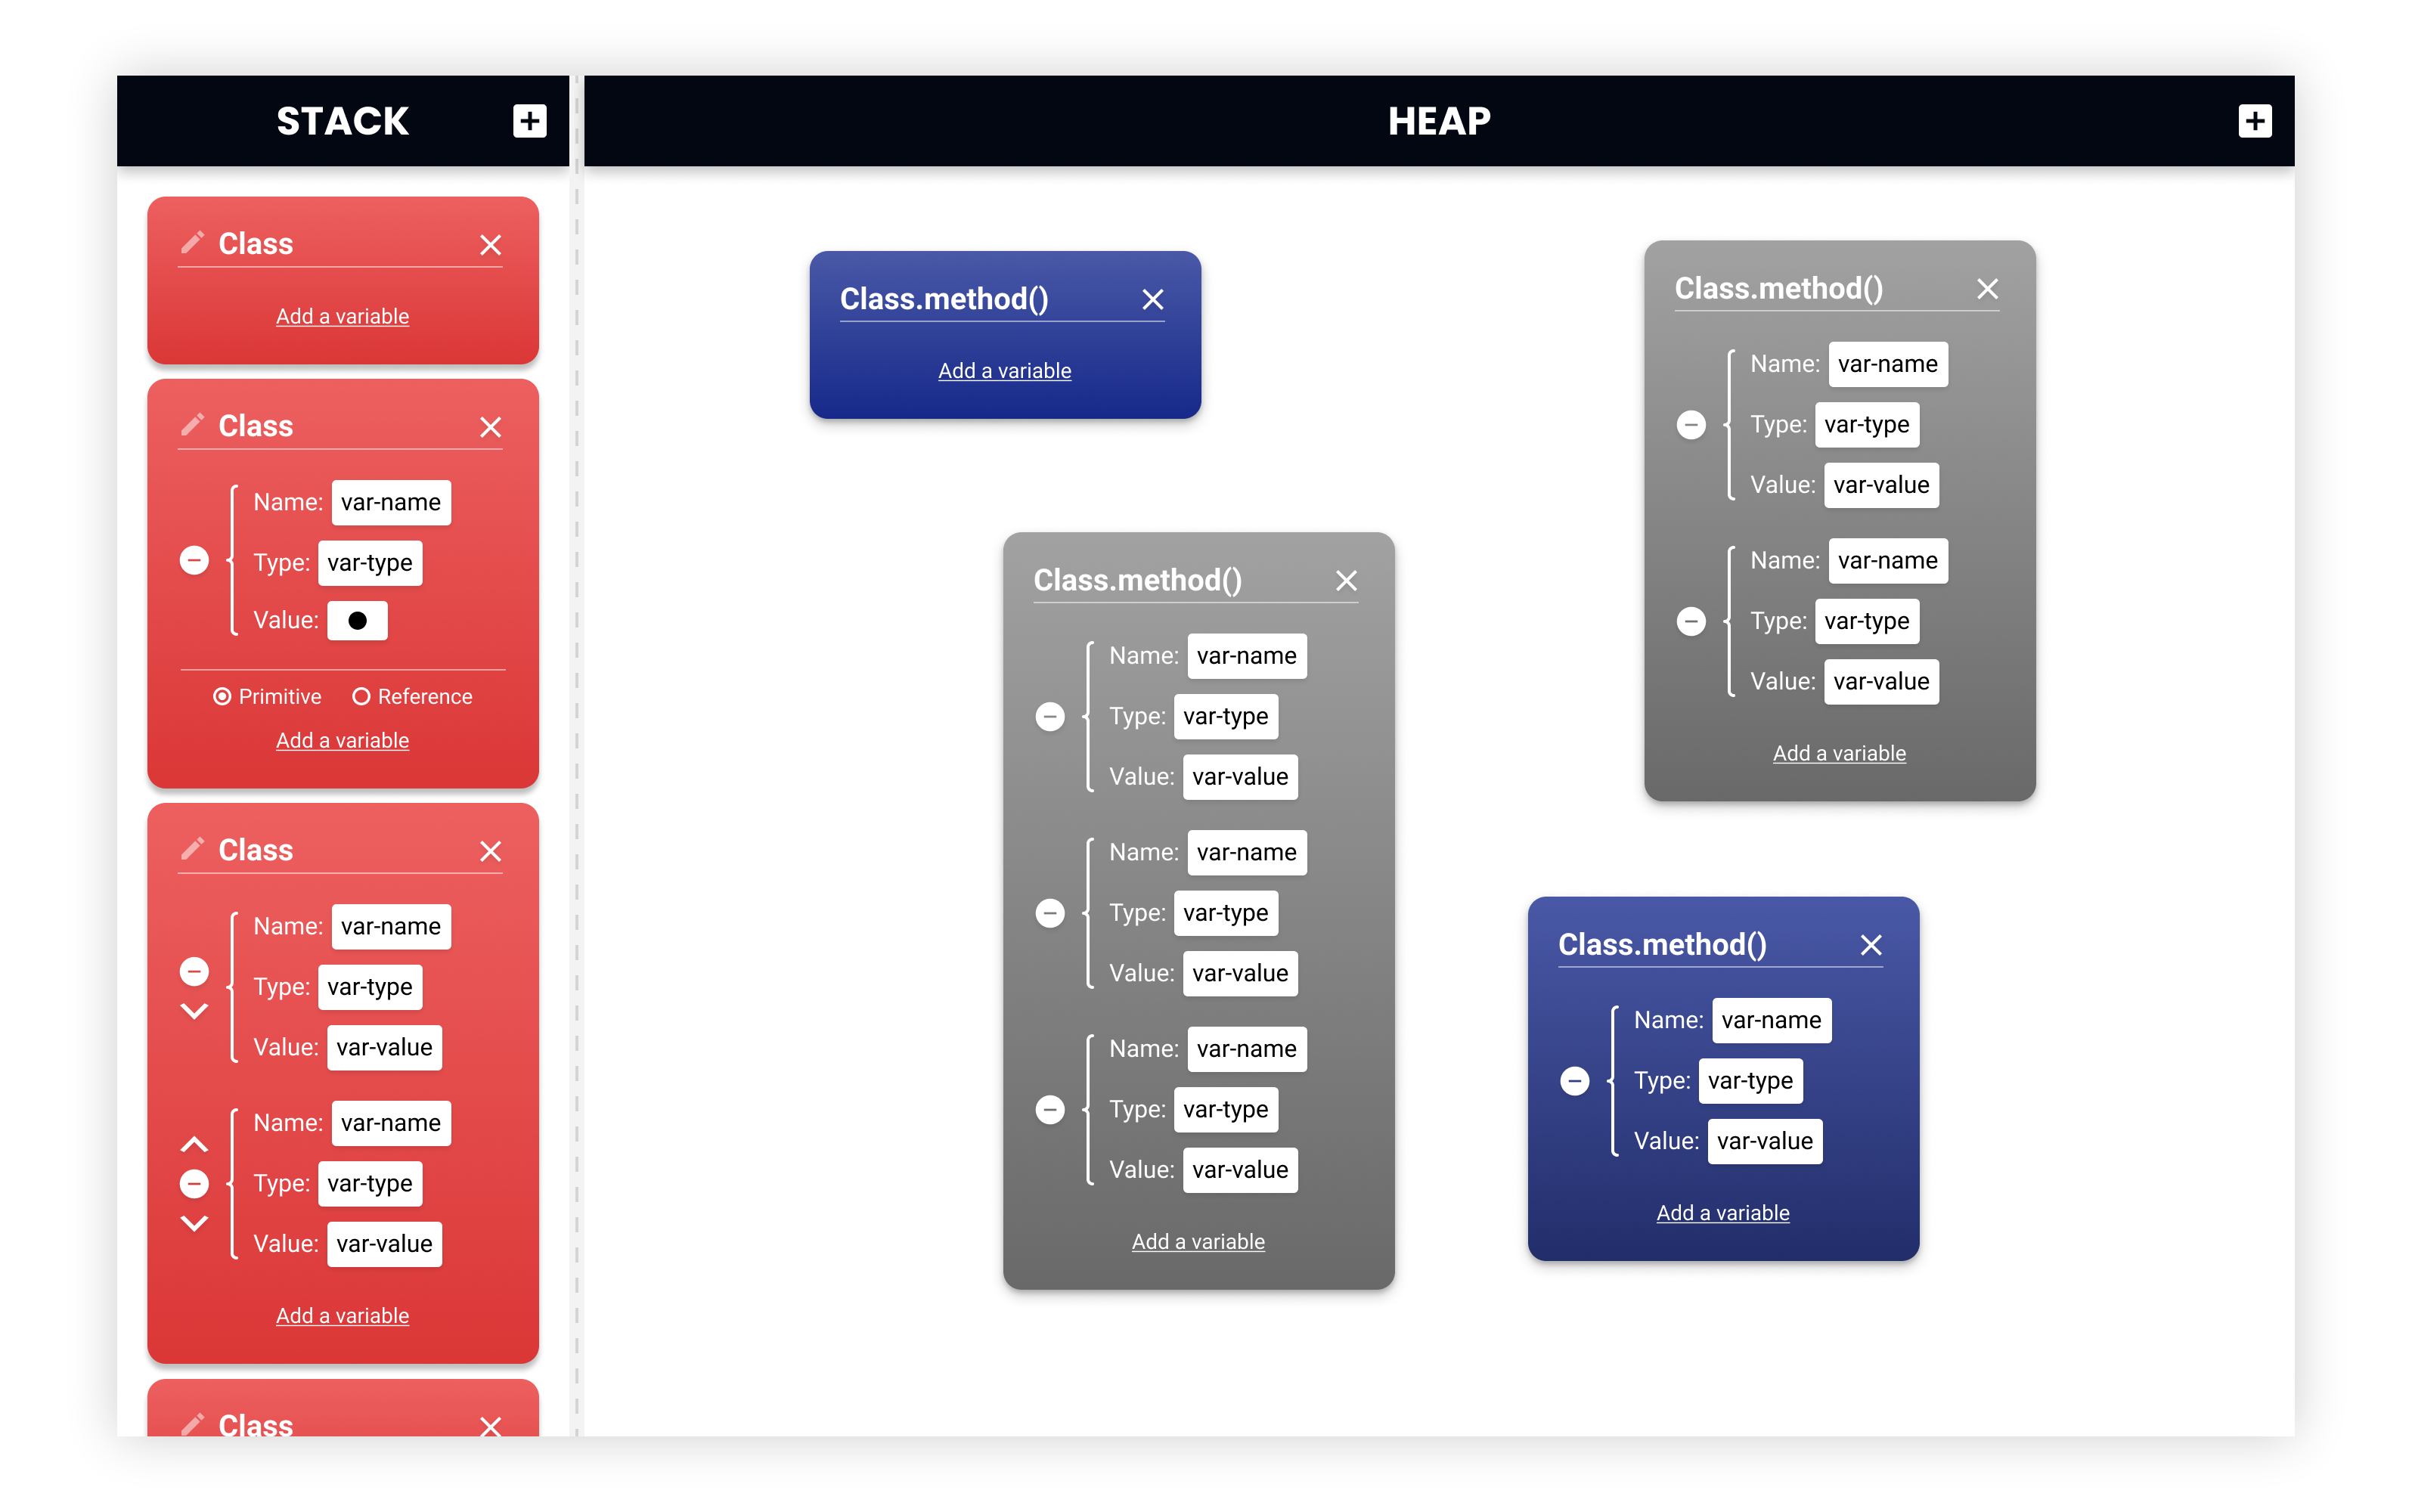
\includegraphics[width=\textwidth]{figures/separate_regions.png}
\caption {Intermediate version of the user interface with separate regions for stack and heap}
\label{separate regions}
\end{figure}

\noindent After several revisions, we eventually found a design solution which was good enough to continue with the rest of the development phase and you can see that in \hyperref[final ui]{\textbf{Figure 9}}. Compared to \hyperref[separate regions]{\textbf{Figure 8}} it presents some clear improvements, such as:

\begin{enumerate}
	\item Redesigned variables. Each one is now represented as a separate box inside the enclosing region block.
	\item Regions headers now display the number of blocks contained in it.
	\item Better color schemes.
	\item A toolbar is now docked on the right side of the window. It can be used to trigger some actions.
	\item Heap objects now have a handle at the top, so that users can drag them around.
\end{enumerate}

\noindent However, at this stage we have also started to notice how blocks were really big as opposed to the ones present in the clicker tool. However, we decided to keep this design because ultimately the pros outnumbered the cons and this issue could have been addressed during development.

\vspace{\fill}

\pagebreak

\begin{figure}[h!]
\centering
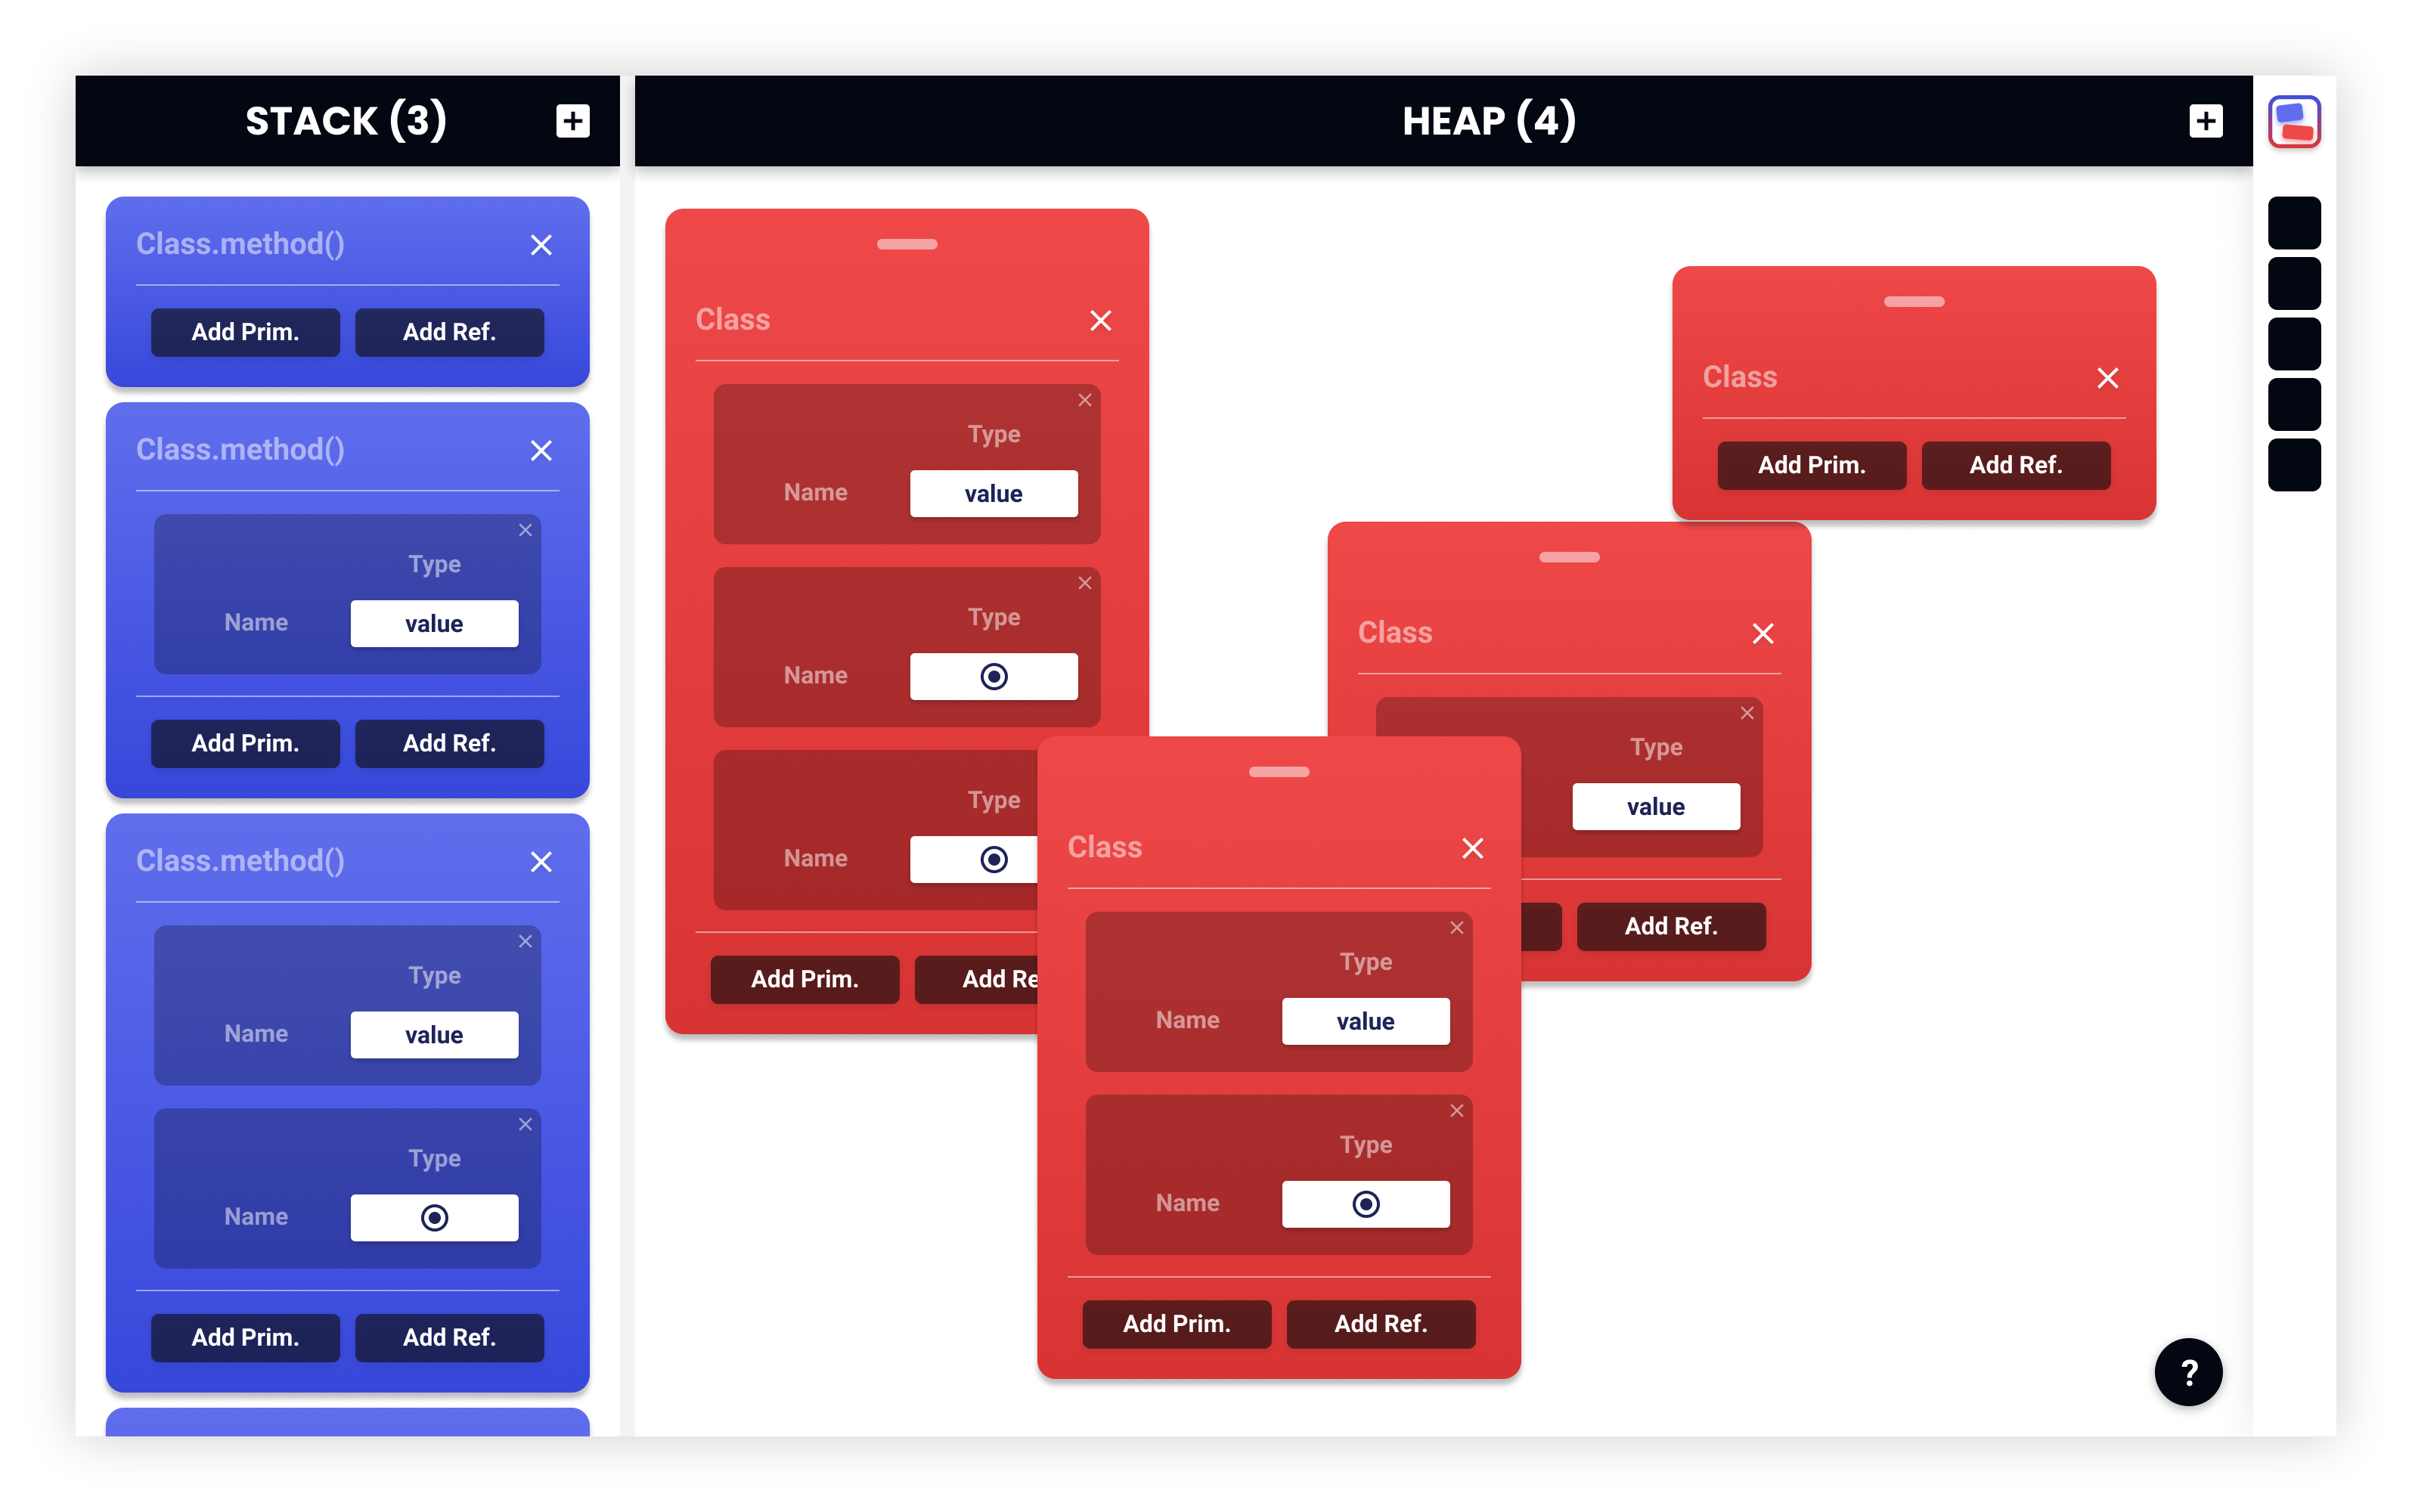
\includegraphics[width=\textwidth]{figures/final_mockup.png}
\caption {Final mockup of the user interface}
\label{final ui}
\end{figure}

\subsection{Components tree}

Although stack and heap are separate regions that expect different user interactions, they share important similarities. In fact, they both:

\begin{itemize}
	\item Have a header, indicating the name of the area and the number of blocks that currently populate it.
	\item Have blocks, which look and function in the exact way, except their color schemes.
\end{itemize}

\noindent Because of these similarities, I have encountered some problems trying to extract the same features in common components in order to avoid as much code repetition as possible (see \hyperref[]{\textbf{Section 5}} for a more detailed explanation about this topic). \hyperref[tree]{\textbf{Figure 10}} shows the components tree on which I eventually settled.

\begin{figure}[h!]
\centering
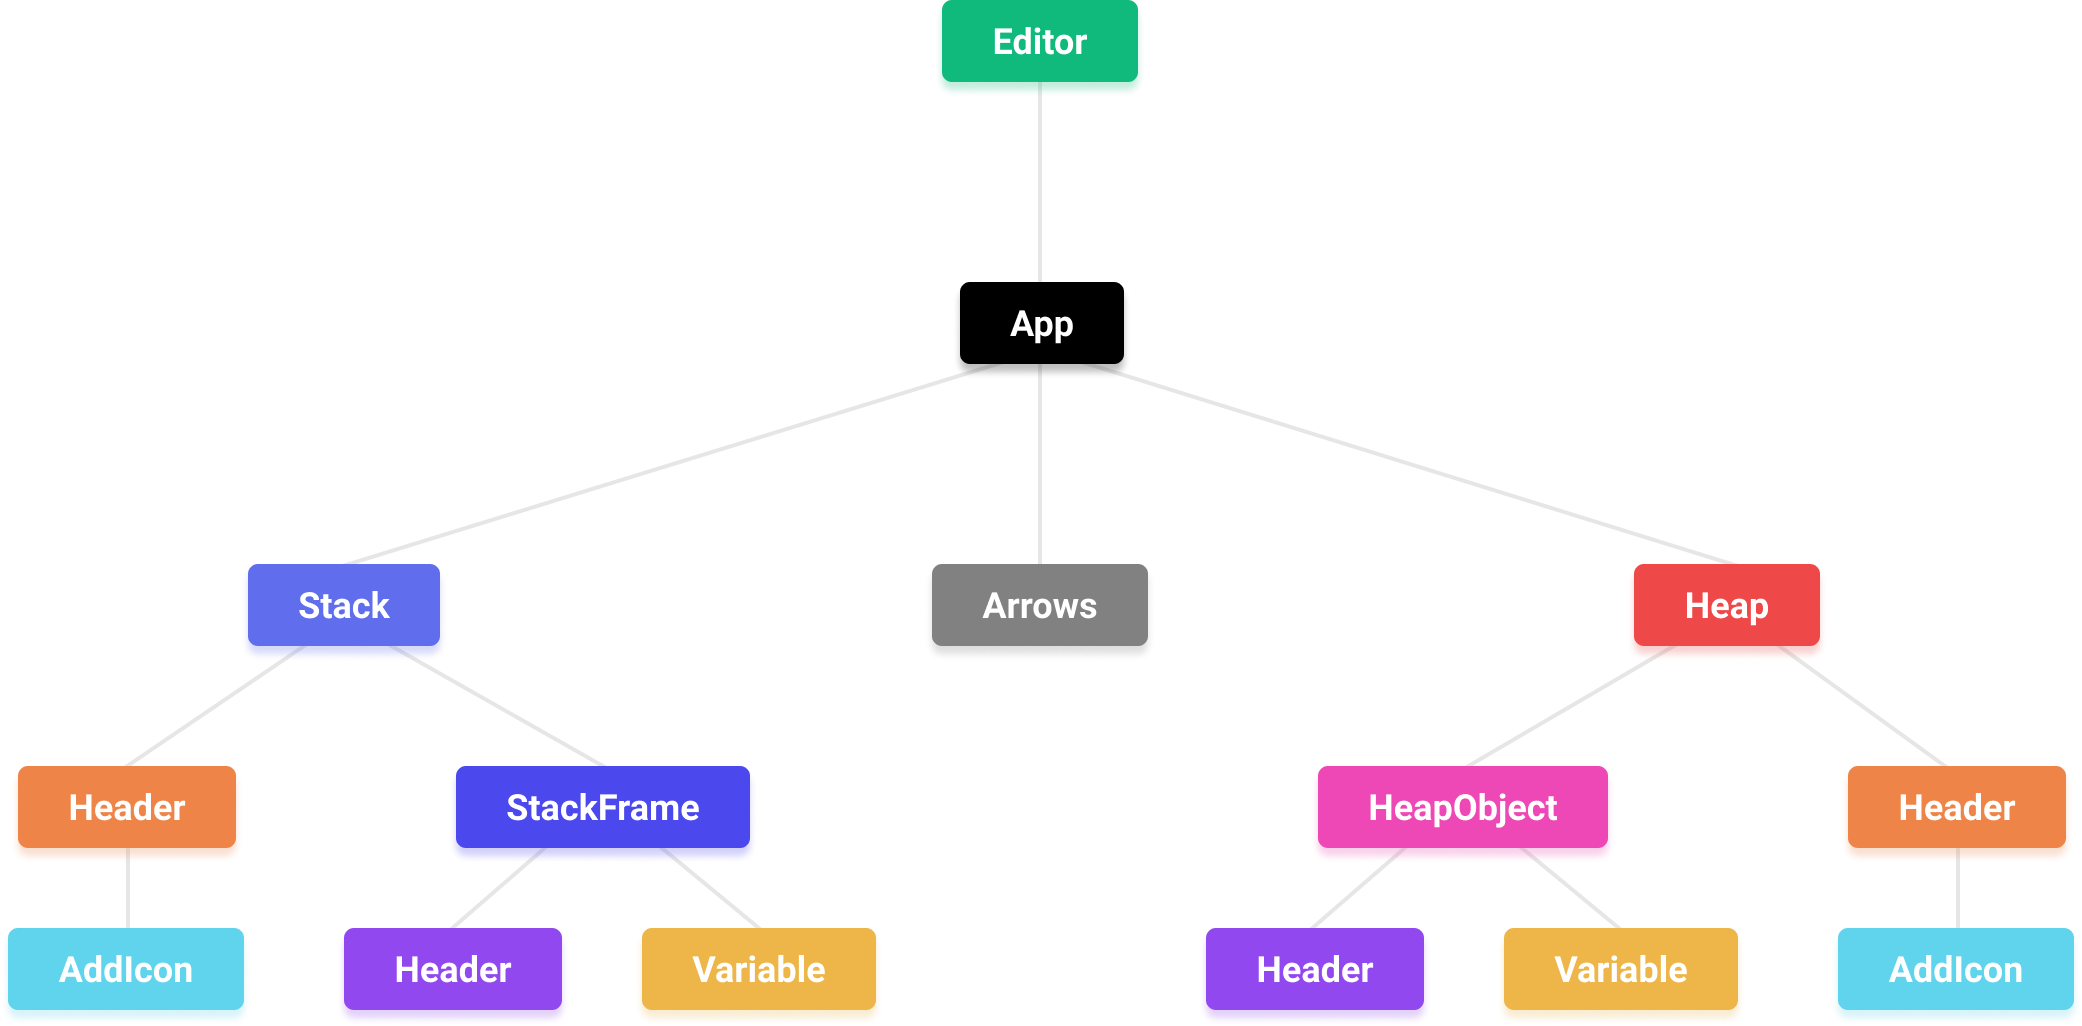
\includegraphics[width=\textwidth]{figures/tree.png}
\caption {Components tree visualization}
\label{tree}
\end{figure}

\pagebreak

\noindent Starting from the top of the tree, \textbf{App} is the highest component and it is mainly used to define the global layout of the web application. Some top-level computations, such as resizing the stack width is done within this component.\\
Following the two branches, \textbf{Stack} and \textbf{Heap} are the components that represent the two areas of memory, and they keep and manage all the information related to their area within the application.\\
If we look at \textbf{\hyperref[tree]{Figure 11}}, we can really see how stack and heap are really similar. In fact, the only difference in their subtrees is the type of building block they can store. The stack stores \textbf{StackFrames}, while heap stores \textbf{HeapObjects}. They look very similar, but the data they generate is different. Here is a snippet of the JSON file created by the web application:\\

\begin{figure}[h!]
\centering
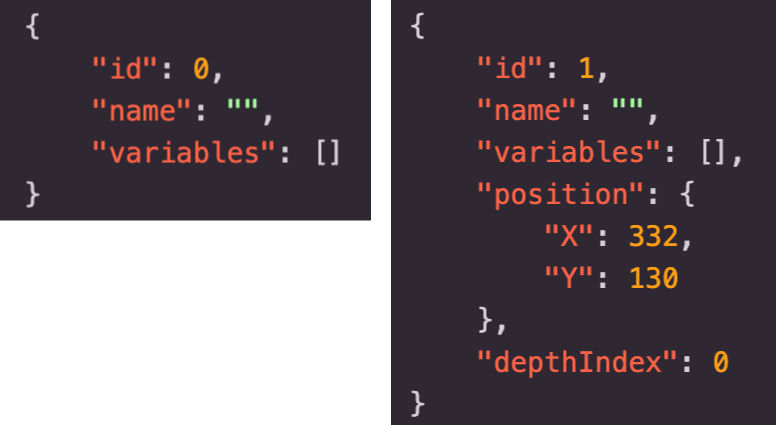
\includegraphics[scale=.3]{figures/blocks_data.png}
\caption {\textbf{Left}: StackFrame, \textbf{Right}: HeapObject}
\label{tree}
\end{figure}

\noindent As we can see, heap objects have more data due to the fact that you can drag them around (hence the \emph{position}) and while doing so the one you are currently moving, goes on top of the other ones (hence the \emph{depthIndex}).\\
Going back to the components tree, every block has a \textbf{Header}, where users can write either the name of the class method name or the class name, and one or more \textbf{Variables}.\\
Both the stack and the heap have a \textbf{Header}, which shows the region name and the number of frames/objects created. Headers at the region level contain a component called \textbf{AddIcon}, which handles the creation of new blocks.

\subsection{UI functionalities}

In this subsection I am going to walk you through every functionality that this stack and heap diagram editor offers to the user.\\

\ul{Stack}

\begin{itemize}
	\item Clicking on the plus button in the header, a new stack frame is created.
	\item Stack frames are always added at the top of the stack.
	\item When the stack contains more frames than the window can fit, the stack becomes scrollable. 
	\item The header renders the number of frames currently populating the stack.
\end{itemize}\

\ul{Heap}

\begin{itemize}
	\item Similarly to what happens in the stack, by clicking on the plus button, users can create new objects on the heap. However, the buttons works a bit differently: when it is yellow, the state is "on", the mouse cursor change and the user can create a new object by clicking on the heap; when it is white, the state is "off" and the objects creation is disabled.
	\item Objects on the heap can be dragged around by clicking on their handle at the top.
	\item In the header it is rendered the number of objects currently populating the heap.
\end{itemize}\

\ul{Regions separator}

\begin{itemize}
	\item Users can drag the vertical separator between the stack and the heap to resize their width.
\end{itemize}

\pagebreak

\ul{Stack frames and heap objects}

\begin{itemize}
	\item Users can type the name of the class method that generated a given stack frame.
	\item Users can type the name of the class that generated a given object on the heap.
	\item Users can create primitive and instance ("reference") variables.
	\item Users can fill the information of a variables, like the name, the type and the value.
	\item If a variable is of nature primitive, its value can be written using the keyboard.
	\item If a variable is of nature reference, an arrow is created by clicking on the circle icon within the value input field, holding the left mouse button and releasing it on a target object on the heap.
\end{itemize}\

\ul{Toolbar}

\begin{itemize}
	\item Users can download a JSON file, representing the current state of the diagram. When pressing this button, a prompt appears to enter the name of this file.
	\item Users can upload a JSON file that was downloaded from the application. This file is parsed and it triggers the application to re-render with the state of the diagram at the time of downloading that file.
	\item Users can start a new project (all stack frames and heap objects are deleted).
	\item Users can scale up the interface. At every click, the base font-size (16px) is increased by 2px.
	\item Users can scale down the interface. At every click, the base font-size (16px) is decreased by 2px.
\end{itemize}

\subsection{Storing global states} \label{storing states}

In React, data is usually shared via props from parent to children: they can receive functions as props and send some data back to the parent using callbacks, but they cannot pass props back to the parent component.\\ Passing props through many levels is called \emph{props drilling} \footnote{\url{https://newreactway.com/what-is-prop-drilling-in-react/}}, and it is generally seen as a situation to avoid if props needs to traverse more than 3 levels of components. In fact, it becomes difficult for the developer to clearly understand what is going on, ending up storing data in intermediate components that are never going to use it.\\

\noindent Depending on the task, there are generally two approaches to solve (or at least improve) the situation:

\begin{enumerate}
	\item Composition
	\item State management tools (e.g., \emph{Redux} \footnote{\url{https://react-redux.js.org/}} and \emph{Context} \footnote{\url{https://reactjs.org/docs/context.html}})
\end{enumerate}

\noindent Both approaches have pros and cons, but for global data transferring it makes more sense to use a state management tool, which is what I did. I used the native React Context API in conjunction with the relatively new \emph{React Hooks} \footnote{\url{https://reactjs.org/docs/hooks-intro.html}}. By doing so, I have been able to access data from any level of tree. However, I must also confess that Context, while being great at what it unlocks, introduces a bit of chaos when overused, which is sadly my case. This is maybe the aspect of this web application I would like to revisit the most in a few years, when I will be more experienced.

\vspace{\fill}

\pagebreak

\noindent In particular I created the following contexts:

\begin{itemize}
	\item \ul{\emph{arrowsContext}}: used to store data about arrows.
	\item \ul{\emph{heapAddModeContext}}: it allows communication between the plus icon in the heap header and the heap dragging area, effectively allowing the user to freely create objects on the mouse position.
	\item \ul{\emph{heapDepthIndexContext}}: it allows me to keep always the current dragged heap object above the others, by correctly setting their css z-index properties.
	\item \ul{\emph{heapMousePositionContext}}: in order to drag heap objects around, many different components needed to access the mouse position, so this context takes care of that.
	\item \ul{\emph{resizableStackContext}}: because of the layout of the application, resizing the stack causes many coordinates to be recomputed, involving components from different  parts of the tree. This context allows all these parties to access the data they need.
	\item \ul{\emph{stateContext}}: this context stores all the data about the diagram and keeps a big JavaScript object updated with every state change happening in the application.
\end{itemize}

\vspace{\fill}

\pagebreak

%%%%%%%%%%%%%%%%%%%%%%%%%
\section{Implementation issues} \label{issues}
%%%%%%%%%%%%%%%%%%%%%%%%%

% 1. Several layers of abstractions
% 2. Several coordinates conversions
% 4. Finding the best compromise between dryness and modularity
% 4. Figuring out how to make the arrows

During the development of this web application, I have faced a few implementation issues. In particular, I had problems of varying degrees with the following points.

\subsection{Multiple coordinates conversions}

At the beginning of the project, when I was building all the JSX and setting up all the CSS rules, I soon discovered that stack and heap needed different "treatments". The stack is built using flexbox with vertical direction, so the coordinates of each stack frame do not really matter, they just stack on top of each other. On the other hand, heap objects need precise coordinates in order to be placed on the screen. However, there is a twist: heap objects coordinates are \emph{relative}, meaning that position ${(0,0)}$ is the top left corner of the heap (header excluded), while mouse coordinates are absolute (= relative to the entire viewport).\\
Objects on the heap use relative coordinates because the stack is resizable: if an object on the heap had position absolute, it would stay in the same place while resizing the stack, not producing the desired effect of seeing everything shift; it would also go \emph{behind} the stack, a very undesirable side effect.\\
Because of that, I often found myself converting coordinates from system to system.

\subsection{Middle ground between dryness and modularity}

In this web app, some components are incredibly similar in term of look but slightly differ in behavior. When using modular frameworks like React, such a situation is not as trivial as one might think. It is very easy to create one single big component that uses conditional rendering in order to avoid code repetition. In my case, that is exactly what happened when I was building the interface and I had just started to work on the drag feature of the objects on the heap.\\ I started having problems when I realized that stack frames and heap objects needed different data representations (i.e. spatial coordinates and z-index values because the current dragged object has to be on top of the other ones). At that point, I had to decouple stack/heap and stack frames/heap objects and find a good compromise between having components with identical elements inside and keep a relatively high level of modularity.

\subsection{Arrows}

Arrows were the toughest feature to implement. Partially because they are implemented using SVG \footnote{\url{https://it.wikipedia.org/wiki/Scalable_Vector_Graphics}} (\emph{Scalable Vector Graphics}) and the syntax and some of its aspect are not very easy (like the path attribute), but also because of their highly dynamic nature in the context of the web application. In fact, in order to render them, I needed to have at least a rudimental system that would register all the information representing an arrow (start/end position, start region, variable and parent from where the connection was created, target object on the heap).\\For that reason, during the first week of work on them, the only way I could have any sort of validation was by constantly printing values on the console in the browser, and by taking and analyzing screenshots. After a while I became very fast and it did not take me long to check on a photo editor if something was correct or not. However, when a bug appeared, the debugging process was always very slow and tedious, because it was difficult to pinpoint the source of the problem.\\

\noindent Another implementation issue I had when working with arrows, was about the way I was updating already drawn arrows. The web application keeps track of two things:

\begin{enumerate}
	\item The new arrow that is being drawn on the screen.
	\item All the arrows that have already been drawn and that need to "listen" for certain events and be updated accordingly (for example, an object that they are connected to, changes its position or gets deleted). When the new arrow is created (the mouse click is released), it gets added to the array if there is not already an arrow with the exact same data. 
\end{enumerate}

\vspace{\fill}

\pagebreak

\noindent When it came down to keep the arrows updated, I could follow two paths:

\begin{enumerate}
	\item Listen for every event that led to the arrow coordinates being recomputed.
	\item Rebuild the whole array of arrows every times the state of the diagram changes.
\end{enumerate}

\noindent Technically, the first approach is more performant, because it only updates the arrows that do really change. However, in such an application it is really unlikely to have so many elements that the performance starts to suffer. Furthermore, using a single point of reference (the state of the diagram) is far easier than watching multiple ones. Hence, I opted for the second way as a solution for this issue \cite{boulay}.


\vspace{\fill}

\pagebreak

%%%%%%%%%%%%%%%%%%%%%%%%%
\section{Testing} \label{Testing}
%%%%%%%%%%%%%%%%%%%%%%%%%

% Methodology can either be:
% 1. User testing -> Users does same task with old and new tool
% 2. Task replication -> I check if everything that was possible with the old tool
%                        still holds up with the new one

\subsection{Methodology}

\subsection{Results}

\subsection{Comments}

\vspace{\fill}

\pagebreak

%%%%%%%%%%%%%%%%%%%%%%%%%
\section{Conclusions} \label{Conclusions}
%%%%%%%%%%%%%%%%%%%%%%%%%

\subsection{Future work}

\vspace{\fill}

\pagebreak

%%%%%%%%%%%%%%%%%%%%%%%%%
% References
%%%%%%%%%%%%%%%%%%%%%%%%%
\bibliographystyle{abbrv}
\bibliography{references}

\end{document}